\documentclass[letterpaper, oneside, final]{memoir}

% packages from file containing all of them
% set up page layout
\setstocksize{11in}{8.5in}
\setlrmarginsandblock{1in}{1in}{*}

\checkandfixthelayout 


% import other packages

\usepackage{amsmath}
\usepackage{amsthm}
\usepackage{amssymb}
\usepackage{graphicx}
\usepackage{hyperref}
\usepackage{csvsimple}
\usepackage{caption}
\usepackage{rotating}

\usepackage[svgnames]{xcolor}
\hypersetup{
    colorlinks,
    linkcolor={DarkBlue},
    citecolor={MediumBlue},
    urlcolor={Blue}
}

\usepackage[sort, numbers, sectionbib]{natbib}
\usepackage{chapterbib}
%\bibliographystyle{abbrvnat}
\renewcommand{\bibname}{References}


\newcommand{\ddx}[2]{\frac{\mathrm{d} #1}{\mathrm{d} #2}}
\newcommand{\pdx}[2]{\frac{\partial #1}{\partial #2}}
\newcommand{\dx}[1]{\mathrm{d} #1 }
\newcommand{\px}[1]{\partial #1 }
\renewcommand{\bar}{\overline}

\newcommand{\mypm}{\mathbin{\smash{%
\raisebox{0.35ex}{%
            $\underset{\raisebox{0.5ex}{$\smash -$}}{\smash+}$%
            }%
        }%
    }%
}

% what chapters to include/compile this time
%\includeonly{ModelVariability/InherentVariabilityChapter}

% document
\begin{document}

\title{Exploring \textit{pyDeltaRCM}: A Collection of Numerical Experiments\\\small{v0.1}}
\author{Jayaram Hariharan}
\maketitle

\tableofcontents

\chapter{Preamble}
\section{Preamble}
``Exploring \textit{pyDeltaRCM}" is a collection of short numerical studies intended to help the reader gain a greater intuition for how the \textit{pyDeltaRCM} model \cite{Moodie2021} behaves.
Each chapter is independent of the others, however all chapters assume basic knowledge of \textit{pyDeltaRCM}.
For background on the \textit{pyDeltaRCM} model and its predecessor, \textit{DeltaRCM}, please refer to \citet{Liang2015a}, \citet{Liang2015}, and \citet{Moodie2021}.
The \textit{pyDeltaRCM} model is open-source software with documentation available at \url{https://deltarcm.org/pyDeltaRCM/} and source-code on GitHub (\url{https://github.com/DeltaRCM/pyDeltaRCM}).\\

\noindent Please contact the authors to further discuss any topics covered within this anthology.

\clearpage
\bibliographystyle{plainnat}
\bibliography{bib/bib}

\chapter{Model Comparison - Original DeltaRCM and pyDeltaRCM}
\section{Background}
DeltaRCM \cite{Liang2015a,Liang2015} is a proven \cite{Liang2015,Liang2016a} and popular \cite{Liang2016,Lauzon2018, Lauzon2019,Piliouras2021} numerical model used to simulate river delta growth and evolution.
The original model was written in MATLAB \cite{MATLAB:R2019b_u4}, leaving room for improvement with regards to code accessibility, run-time, documentation, parallelization, and extensibility.
With these needs in mind, a Python \cite{PythonSoftwareFoundation2016} implementation of the original DeltaRCM model was developed, dubbed \textit{pyDeltaRCM} \cite{Moodie2021}.
This re-implementation of the DeltaRCM model includes minor modifications to the original DeltaRCM methods, and so there is a need to compare the new \textit{pyDeltaRCM} model outputs to those from the original DeltaRCM code. 
In this chapter, this model-to-model comparison is performed using a suite of 35 model runs from each version of DeltaRCM.
The similarities and differences between the two models are quantitatively assessed using a small collection of metrics.

\section{Modeled Scenarios}
Seven scenario are modeled to simulate 200 years of river delta growth into an empty basin assuming 10 bankfull days of discharge per year.
For each scenario, 5 replicate runs are conducted to capture the range of stochastic variability present due to the random walk-based methodology.

\subsection{Parameter Set}
A comprehensive although non-exhaustive list of the model parameter values used for both the MATLAB and Python simulations is provided in Table \ref{tab:params}.

\begin{table}[!ht]
\begin{center}
\begin{tabular}{| c | c | c | c | c |}
\hline
Parameter & Value \\
\hline
dx & 50 m \\
L0 & 150 m \\
Np\_water & 2000 \\
Np\_sed & 2000 \\
u0 & 1 m/s \\
N0 & 250 m \\
h0 & 5 m \\
H\_SL & 0 m \\
f\_bedload & 0.2 \\
C0\_percent & 0.1 \\
Csmooth & 0.9 \\
omega\_sfc & 0.1 \\
omega\_flow & 0.9 \\
Nsmooth & 10 \\
theta\_water & 1 \\
coeff\_theta\_sand & 2 \\
coeff\_theta\_mud & 1 \\
beta & 3 \\
sed\_lag (lambda) & 1 \\
coeff\_U\_dep\_mud & 0.3 \\
coeff\_U\_ero\_mud & 1.5 \\
coeff\_U\_ero\_sand & 1.05 \\
alpha & 0.1 \\
\hline
\end{tabular}
\caption{Model Parameters}
\label{tab:params}
\end{center}
\end{table}

The 7 modeled scenarios simulate different levels of steady sea level rise (SLR).
These 7 SLR values are 0, 5, 10, 15, 20, 30, and 40 mm/yr.
Rates of SLR are scaled temporally under the assumption that the model is simulating 10 bankfull days of discharge per year.

A low value for \texttt{f\_bedload} (20\% sand) is used in these simulations as low sand content generates highly cohesive and more variable simulation results.
High input sand fraction values will result in simulations with smoother deltas.
For the purposes of comparing models, it should be easier to detect differences between rougher planform shapes than smooth ones.


\subsection{Parameter Differences}
The interval at which model outputs are saved was different between the models. For the MATLAB code, saving occurs every 25 model timesteps, whereas in the Python code the model is saved every 35 timesteps.
The save interval does not impact the model behavior, but rather our ability to observe what the model is doing.

The modeled domain size is different between the two sets of runs performed, although in neither case do the simulated deltas reach the domain boundaries.
In the MATLAB scenarios the basin is 9 km long and 17 km wide.
In the Python scenarios the basin is slightly larger with a length of 10 km and a width of 20 km.

Two model parameters are set to slightly different values in these sets of model runs.
The reference slope, \texttt{S0}, is $1.4 \times 10^{-4}$ for the MATLAB model runs, and $1.5 \times 10^{-4}$ for the Python model runs.
The number of times the water parcel routing occurs per timestep, \texttt{itermax}, differs between the runs.
In the MATLAB models \texttt{itermax} $=1$, as this is a computationally expensive step because the water parcels are routed in serial.
The Python models use \texttt{itermax} $=3$, as the new version of the model now routes all of the water parcels in parallel making this step much faster. 

\section{Topographies}
Topography at the end of model runs (after 200 years), is shown in Figure \ref{fig:finaltopo}.
A break in the colorbar to distinguish between water and land is made at 0.5 m below sea level based on color palettes used in previous studies \cite{Liang2016a, Liang2016}.

\begin{figure}[!ht]
	\makebox[\textwidth][c]{
	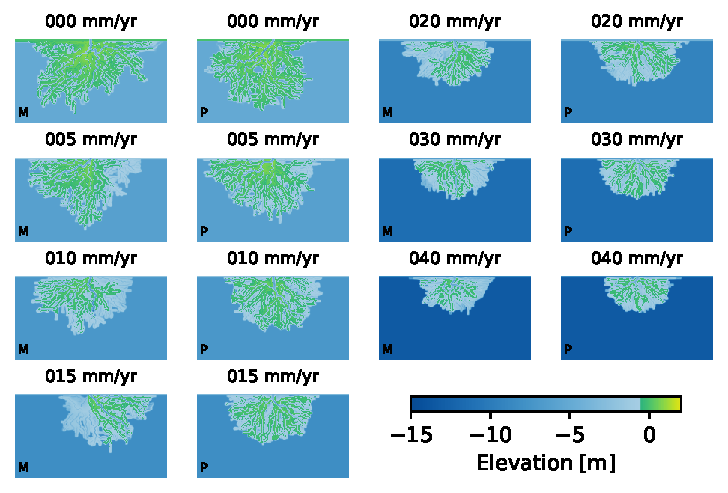
\includegraphics[width=\textwidth]{DeltaRCM_ModelComparison/figs/FinalTopo.pdf}
	}
	\caption{Single model realization final topographies. Numerical model used indicated by letter in bottom left corner of each plot, M for MATLAB and P for Python. Note that the domain has been clipped in all images.}
	\label{fig:finaltopo}
\end{figure}

\section{Metrics}

\subsection{Surface Morphology}

\subsubsection{Planform Area}
The area of the delta planform is identified using a topographic threshold of 0.5 m below the sea level \cite{Liang2016a,Liang2016} and the opening angle method \cite{Shaw2008} with an opening angle of $75^{\circ}$.

\begin{figure}[!htbp]
	\makebox[\textwidth][c]{
	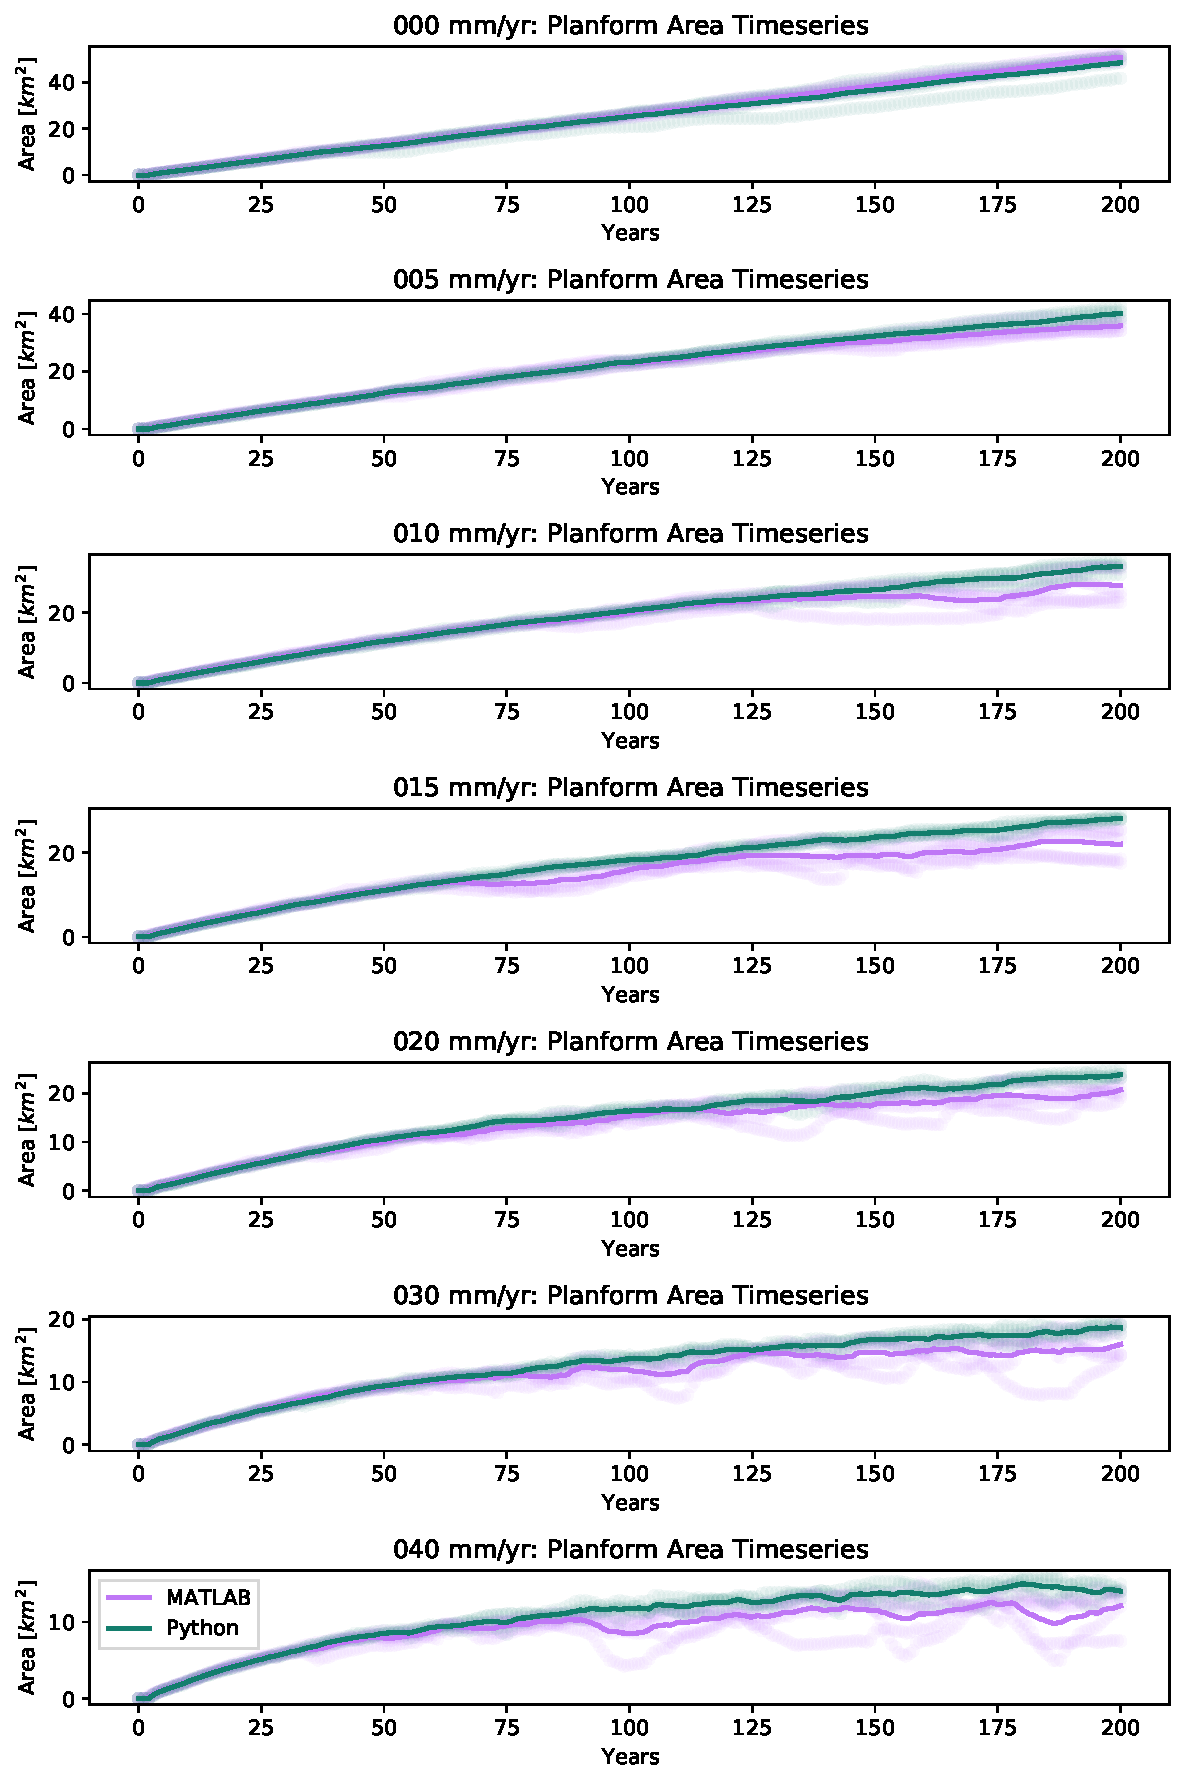
\includegraphics[height=\textheight]{DeltaRCM_ModelComparison/figs/Area.pdf}
	}
	\caption{Planform area timeseries with average values shown as lines and individual run results shown as faint circles. MATLAB results shown in light purple, Python results in dark green.}
	\label{fig:area}
\end{figure}

\subsubsection{Channelized Fraction}
The channelized pixels on the delta topset are identified as locations where the water velocity exceeds the threshold for sediment mobilization (0.3 m/s) \cite{Liang2016a,Liang2016,Lauzon2018,Lauzon2019}.
Then, the channelized fraction is computed by dividing the channelized area by the total area of the topset (the planform area).

\begin{figure}[!htbp]
	\makebox[\textwidth][c]{
	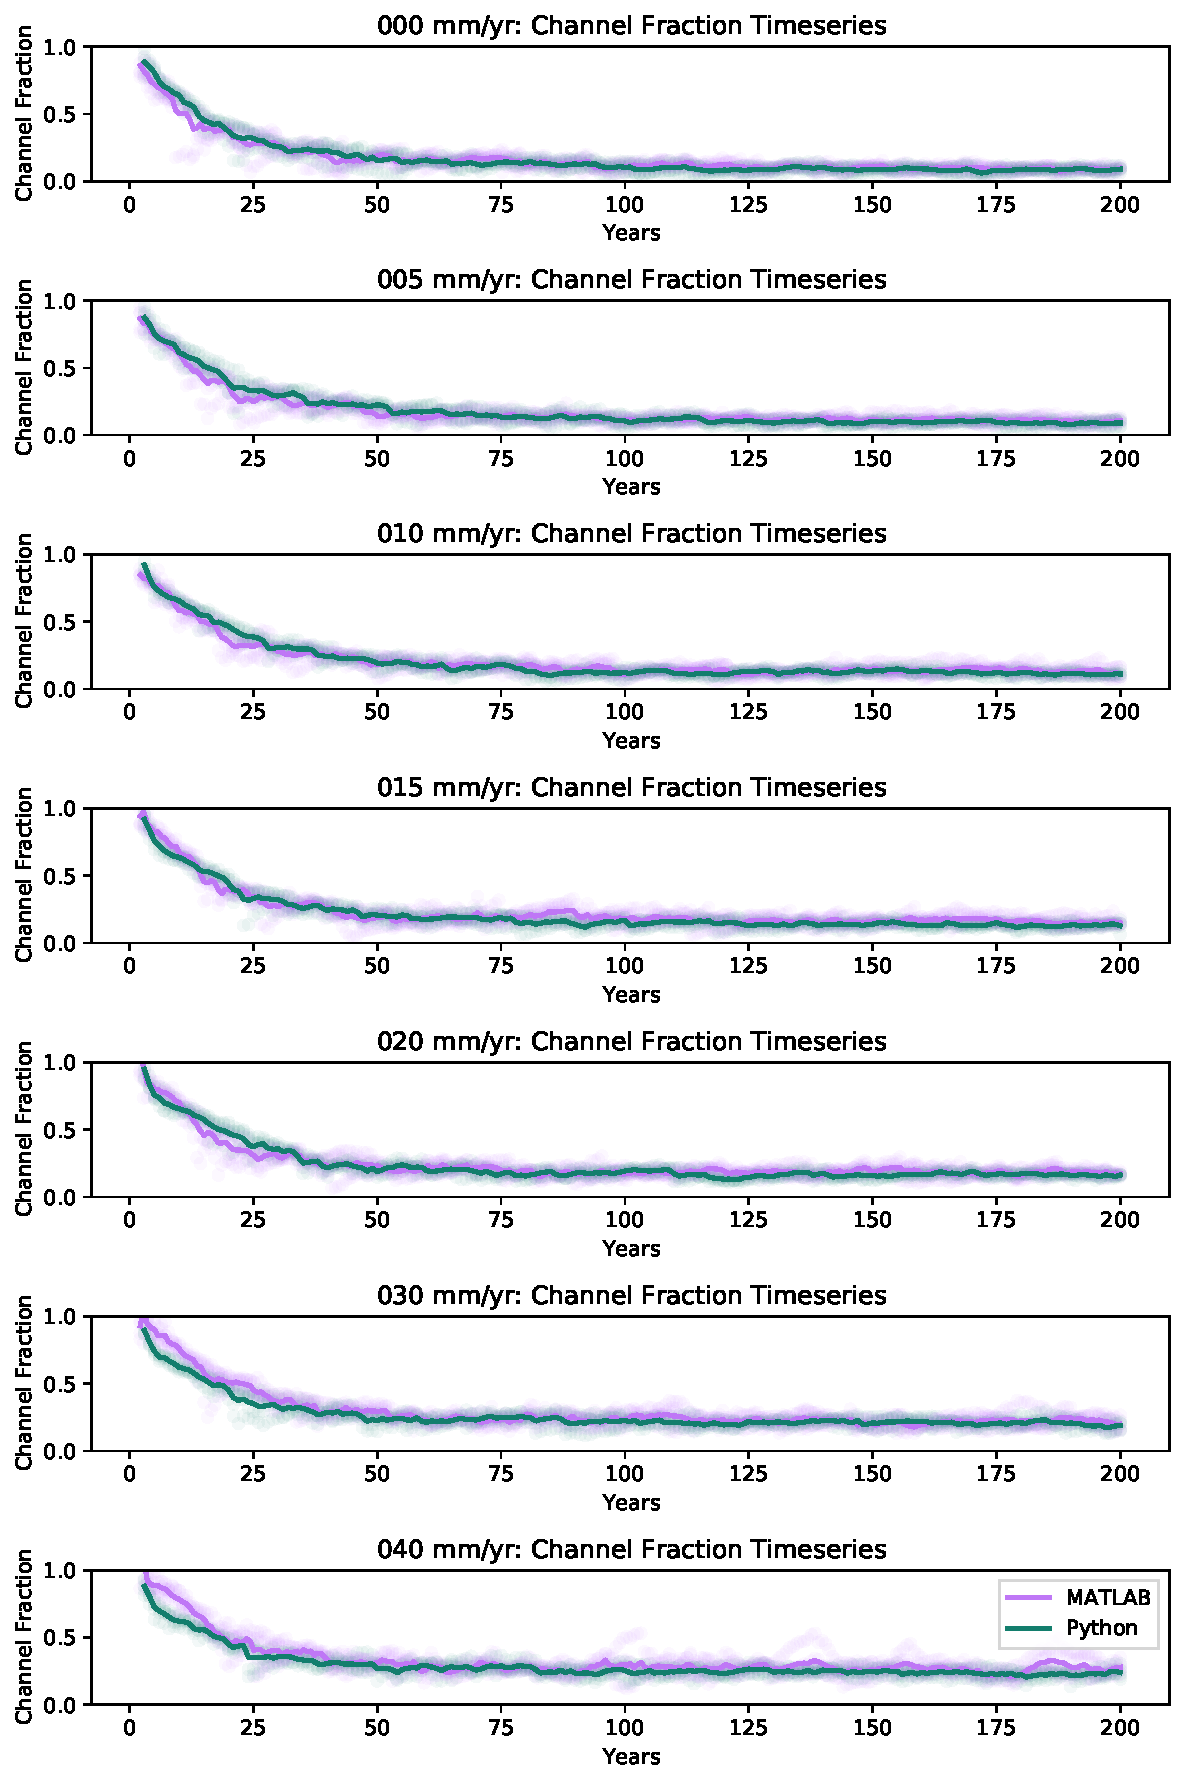
\includegraphics[height=\textheight]{DeltaRCM_ModelComparison/figs/ChannelDensity.pdf}
	}
	\caption{Channelized fraction timeseries with average values shown as lines and individual run results shown as faint circles. MATLAB results shown in light purple, Python results in dark green.}
	\label{fig:channelfraction}
\end{figure}

\subsubsection{Shoreline Roughness}
Shoreline roughness is calculated as the length of the shoreline divided by the square root of the planform area.
The shoreline is derived from the land map of the delta planform by performing morphological operations using the scikit-image Python library \cite{scikit-image}.
First edge detection \cite{roberts1963machine} is performed, and then the resulting edge is made binary and skeletonized \cite{zhang1984fast}, defining the shoreline.

\begin{figure}[!htbp]
	\makebox[\textwidth][c]{
	\includegraphics[height=\textheight]{DeltaRCM_ModelComparison/figs/ShoreRough.pdf}
	}
	\caption{Shoreline roughness timeseries with average values shown as lines and individual run results shown as faint circles. MATLAB results shown in light purple, Python results in dark green.}
	\label{fig:shorelineroughness}
\end{figure}

\subsection{Surface Dynamics}

\subsubsection{Channel Planform Overlap}
The channel planform overlap metric \cite{Wickert2013} measures the loss of similarity in channel locations over time.
It is common for the normalized overlap value, $O_{\Phi}$, to be used to fit an exponential decay equation
\begin{equation}
O_\Phi = \left(a_M - p_M\right) e^{-Mt} + p_M,
\end{equation}
where $M$, the decay constant (units of inverse time), is a mobility parameter describing how quickly the channel system is reworking itself.
For these 200 year simulations, the channel planform overlap is evaluated using base channel maps from recorded outputs in the interval [100, 150] years.
These base maps are compared to those within 50 years, meaning the transient maps are sourced from the interval (100, 200] years.

%\csvautotabular{tables/MATLAB_mobilitydata.csv}

\begin{table}[!ht]
\begin{center}
\begin{tabular}{| c | c | c | c |}
\hline
SLR [mm/yr] & $a_M$ & $M$ [yr$^{-1}$] & $p_M$ \\
\hline
\hline
\csvreader[late after line=\\\hline]
   {DeltaRCM_ModelComparison/tables/MATLAB_mobilitydata.csv}{SLR [mm/yr]=\slr, $a_M$=\am, $M$=\m, $p_M$=\pm}
   {\slr & \am & \m & \pm}
\end{tabular}
\caption{MATLAB planform overlap exponential fit parameters. Average parameter values for the set of 5 replicate runs reported $\mypm$ the average standard deviation of the individual parameter estimates.}
\label{tab:RCMmobility}
\end{center}
\end{table}

\begin{table}[!ht]
\begin{center}
\begin{tabular}{| c | c | c | c |}
\hline
SLR [mm/yr] & $a_M$ & $M$ [yr$^{-1}$] & $p_M$ \\
\hline
\hline
\csvreader[late after line=\\\hline]
   {DeltaRCM_ModelComparison/tables/Python_mobilitydata.csv}{SLR [mm/yr]=\slr, $a_M$=\am, $M$=\m, $p_M$=\pm}
   {\slr & \am & \m & \pm}
\end{tabular}
\caption{Python planform overlap exponential fit parameters. Average parameter values for the set of 5 replicate runs reported $\mypm$ the average standard deviation of the individual parameter estimates.}
\label{tab:Pymobility}
\end{center}
\end{table}

%\subsubsection{Channel Abandonment}
%Channel abandonment is calculated using the number of channelized pixels from some base map which remain channelized at later times \cite{Liang2016}.
%To this decay curve, a harmonic function is fit \cite{Cazanacli2002}, formulated as,
%\begin{equation}
%f_{remain} = \frac{f_0}{1 + \frac{t}{t_{rw}}},
%\end{equation}
%where $t_{rw}$ represents a characteristic decay time for the abandonment of the channel.

\subsection{Subsurface Composition}

\subsubsection{Net-to-Gross Ratio}
The net-to-gross ratio of the total deposit is calculated as the sum of sand fraction values in the preserved stratigraphy divided by the total number of voxels in the stratigraphy.
Stratigraphy in both models is computed at a vertical resolution of 5 cm.

\begin{table}[!ht]
\begin{center}
\begin{tabular}{| c | c | c | c | c | c | c | c |}
\hline
SLR [mm/yr] & Run 1 & Run 2 & Run 3 & Run 4 & Run 5 & \textbf{Avg.} & Std. Dev. \\
\hline
\hline
\csvreader[late after line=\\\hline]
   {DeltaRCM_ModelComparison/tables/MATLAB_netgross.csv}{SLR [mm/yr]=\slr, Run 1=\a, Run 2=\b, Run 3=\c,
   								Run 4=\d, Run 5=\e, Avg.=\avg, Std. Dev.=\std}
   {\slr & \a & \b & \c & \d & \e & \bfseries\avg & \std}
\end{tabular}
\caption{MATLAB net-to-gross values}
\label{tab:RCMnetgross}
\end{center}
\end{table}

\begin{table}[!ht]
\begin{center}
\begin{tabular}{| c | c | c | c | c | c | c | c |}
\hline
SLR [mm/yr] & Run 1 & Run 2 & Run 3 & Run 4 & Run 5 & \textbf{Avg.} & Std. Dev. \\
\hline
\hline
\csvreader[late after line=\\\hline]
   {DeltaRCM_ModelComparison/tables/Python_netgross.csv}{SLR [mm/yr]=\slr, Run 1=\a, Run 2=\b, Run 3=\c,
   								Run 4=\d, Run 5=\e, Avg.=\avg, Std. Dev.=\std}
   {\slr & \a & \b & \c & \d & \e & \bfseries\avg & \std}
\end{tabular}
\caption{Python net-to-gross values}
\label{tab:Pynetgross}
\end{center}
\end{table}

%\subsubsection{Downstream Fining}
%To obtain some measure of the spatial partitioning of sediment within the deposit, the notion of downstream fining will be explored.

\section{Statistical Tests}

\subsection{Rank-Sum Tests}
Results for the channelized fraction and shoreline roughness metrics are qualitatively stationary in time after the initial channel network is formed (Figures \ref{fig:channelfraction} \& \ref{fig:shorelineroughness}).
The DeltaRCM channel network may form in as few as 75 years \cite{Liang2016a, Lauzon2018, Lauzon2019, Piliouras2021}.
Therefore, metric values between years 100 and 200 reflect properties of the fully developed distributary network.
Values from the 5 replicates per SLR scenario are lumped together for each model (MATLAB and Python), and used to perform a rank-sum test \cite{wilcoxon1945} with a null hypothesis, $H_0$: the two sets of values are drawn from the same distribution.

\begin{table}[!ht]
\begin{minipage}[b]{0.3\linewidth}
\centering
\begin{tabular}{| l | r |}
\hline
SLR [mm/yr] & p-value \\
\hline
\hline
\csvreader[late after line=\\\hline]
   {DeltaRCM_ModelComparison/tables/channeldensity.csv}{SLR [mm/yr]=\slr, p-value=\pv}
   {\slr & \pv}
\end{tabular}
\caption{Channel Fraction Rank-Sum Results}
\label{tab:chanfrac}
\end{minipage}\hfill
\begin{minipage}[b]{0.65\linewidth}
\centering
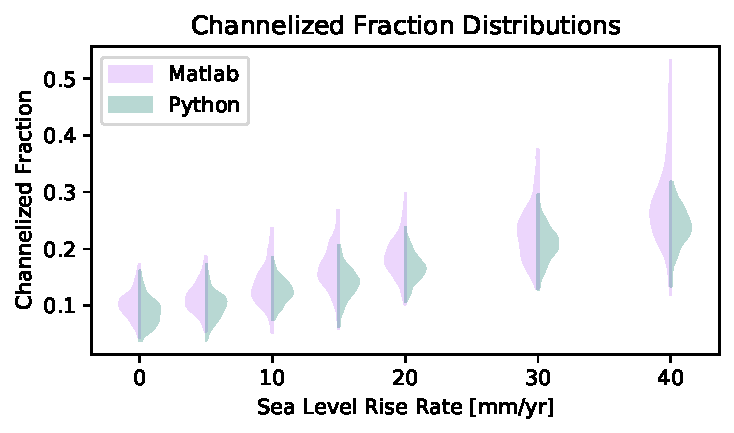
\includegraphics[width=3.5in]{DeltaRCM_ModelComparison/figs/ChannelFracDists.pdf}
\captionof{figure}{Smoothed distributions of channel fraction values (years 100-200).}
\label{fig:chanfrac}
\end{minipage}
\end{table}

\begin{table}[!ht]
\begin{minipage}[b]{0.3\linewidth}
\centering
\begin{tabular}{| l | r |}
\hline
SLR [mm/yr] & p-value \\
\hline
\hline
\csvreader[late after line=\\\hline]
   {DeltaRCM_ModelComparison/tables/shorelineroughness.csv}{SLR [mm/yr]=\slr, p-value=\pv}
   {\slr & \pv}
\end{tabular}
\caption{Shoreline Roughness Rank-Sum Results}
\label{tab:shorerough}
\end{minipage}\hfill
\begin{minipage}[b]{0.65\linewidth}
\centering
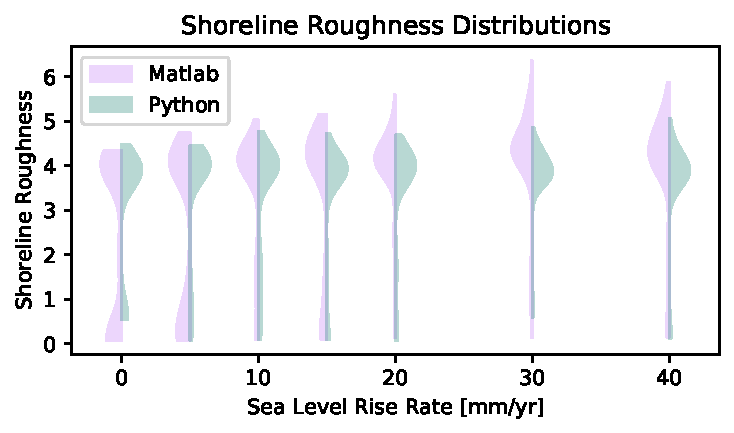
\includegraphics[width=3.5in]{DeltaRCM_ModelComparison/figs/ShoreRoughDists.pdf}
\captionof{figure}{Smoothed distributions of shoreline roughness values (years 100-200).}
\label{fig:shorerough}
\end{minipage}
\end{table}

%\subsection{Kruskal-Wallis Tests}
%Treat each individual set of results from a single model replicate as an independent group.
%Test null hypothesis that all of the 10 groups for a given scenario (5 from MATLAB, 5 from Python) have identical distributions.

\section{Conclusions}
Although model results look qualitatively very similar, there are some slight differences between the MATLAB and Python outputs.
It is hard to know whether or not these differences are due to the differences in parameter values for \texttt{S0} and \texttt{itermax}, or whether they are due to actual code differences.
It is harder still to know whether or not these differences matter and which model is generally more representative of true systems and processes.

On the surface, the channelized fraction (Figure \ref{fig:channelfraction}) and shoreline roughness (Figure \ref{fig:shorelineroughness}) appear to be similar between the models, however a rank-sum test performed comparing the values from years 100-200 (Tables \ref{tab:chanfrac} \& \ref{tab:shorerough}), suggest that the underlying distributions are indeed different.

The surface dynamics, as measured using the channel planform overlap metric, provide evidence of similar trends between the two models (increasing mobility with increasing sea level rise rates).
However, the Python implementation appears to be more mobile than the MATLAB version (Tables \ref{tab:RCMmobility} \& \ref{tab:Pymobility}, third column).
This trend in particular may be influenced by the frequency at which model outputs were obtained, the MATLAB code output information about the system every 25 timesteps ($\sim0.7$ years) whereas the Python code was set to output information every 35 timesteps ($\sim1$ years).

Net-to-gross properties of the preserved deposits also present slightly perplexing results.
The MATLAB results show a deposit that tends to be sandier than the input bedload fraction, with increasing sandiness with higher sea level rise rates (Table \ref{tab:RCMnetgross}).
On the other hand, the Python results show an opposite trend, with decreasing sandiness as the sea level rise rate is increased, and overall net-to-gross values at or slightly below the input bedload fraction (Table \ref{tab:RCMnetgross}).

\clearpage
\bibliographystyle{plainnat}
\bibliography{bib/bib}

\chapter{Runtime Variability}
\section{Background}
The reduced-complexity approach to delta modeling employed in \textit{pyDeltaRCM} hinges upon the notion of the random walk \cite{Pearson1905}.
To approximate physics, the DeltaRCM methodology does not use a truly random walk and rather weights the transport pathways of water and sediment to approximate physical processes.
As a result, an individual model run represents a single stochastic realization for a given parameter set. 
The variability in the model run behavior is also expected to result in runtime variability.
Understanding the variability in run times for any given set of model parameters can help estimate the required computational time to conduct a set of numerical experiments and can also be used to set wall-clock times for model runs conducted on HPC clusters. 

\section{Model Runs}
A set of 100 small model runs are conducted to develop an understanding of the variability in model run time for a fixed set of parameters.
The following YAML file is used to conduct the model runs.
For these realizations a special subclass of the standard \textit{pyDeltaRCM} model is used which tracks and records the number of sediment parcel iterations conducted in each realization.
The underlying hypothesis is that the sediment parcel iteration process consumes the majority of the model runtime, and therefore one would expect to see a correlation between the number of sediment parcel iterations and the runtime for any given realization.\\

\noindent \texttt{YAML} configuration file: \vspace{-6pt}
\begin{boxedverbatim}
timesteps: 1500
ensemble: 100
Length: 4000.0
Width: 7000.0
dx: 50.0
L0_meters: 50.0
u0: 1.0
N0_meters: 250.0
h0: 5.0
save_dt: 250000
save_metadata: True
save_eta_grids: True
SLR: 48e-10  # small background SLR
f_bedload: 0.5
\end{boxedverbatim}

\section{Results}
The 100 runs completed with an average runtime of 2.025 hours per run, and a standard deviation of 0.082 hours. 
A histogram of the runtimes for the 100 runs with a kernel-density estimated smoothed PDF overlaid is provided (Figure \ref{fig:runtimes}, second row).
These results reveal a disparity of about 0.5 hours between the slowest and the fastest realization, significant ($\sim25\%$) in the context of runs that are taking an average of just 2 hours to complete. 

\begin{figure}[!ht]
	\makebox[\textwidth][c]{
	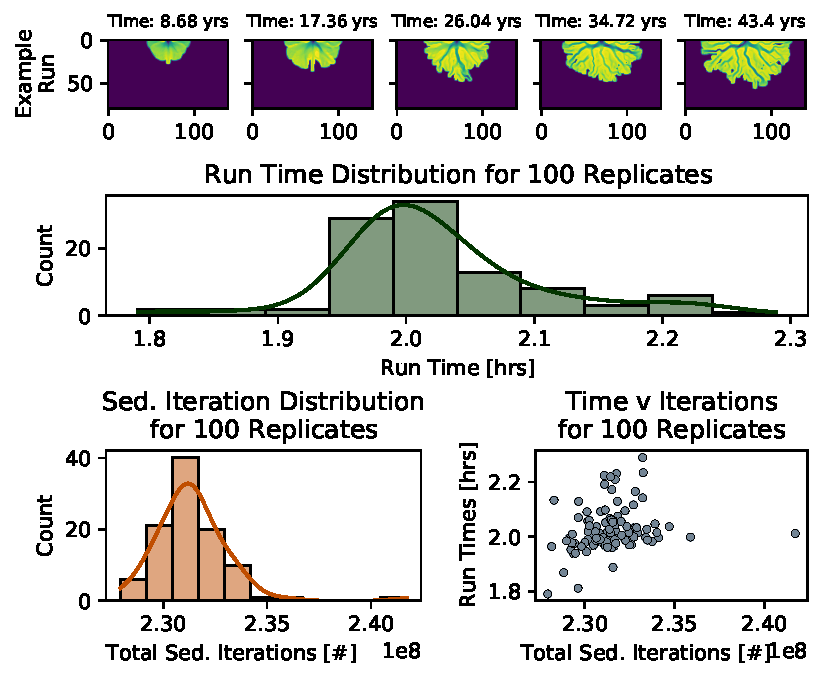
\includegraphics[width=\textwidth]{RuntimeVariability/figs/runtimes.pdf}
	}	
	\caption{Results from the 100 runs generated by the YAML configuration file. \textit{Top row:} Evolution of model topography from a single realization. \textit{Second row:} Run time distribution for the 100 runs, histogram shown with Kernel Density Estimated PDF. \textit{Bottom Left:} Distribution of the total sediment parcel iterations for the 100 runs. \textit{Bottom Right:} Cross-plot of the 100 model run times against the total sediment parcel iterations.}
	\label{fig:runtimes}
\end{figure}

\section{Conclusions}
There appears to be a non-negligible degree of variability in the run times for different realizations run from the same parameter set.
This variability is not directly linked to the number of sediment parcel iterations, as a strong correlation between run time and total sediment parcel iterations does not exist (Figure \ref{fig:runtimes}, bottom right).
When planning a set of numerical experiments, if one or two prototype runs have been conducted to test the parameter set and the size of the domain, the computational time required to conduct a larger ensemble of runs can be estimated conservatively by inflating the prototype run times by $\sim25\%$ and multiplying that value by the number of simulations being run.

\clearpage
\bibliographystyle{plainnat}
\bibliography{bib/bib}

\chapter{Grid Resolution and Model Runtime}
\section{Background}
Understanding the relationship between cell resolution ($dx$) and model run time is extremely helpful when designing future numerical experiments.
This relationship has been hypothesized, but is unknown with regards to the \textit{pyDeltaRCM} model (at the time of writing). 

\section{Model Runs}
A set of 6 model runs, each with a different cell resolution ($dx$) are conducted.
These runs are at ``field-scale" using parameters similar to those from previous studies \cite{Liang2016, Liang2016a}.
The YAML below provides information about the parameter set used.\\

\noindent \texttt{YAML} configuration file: \vspace{-6pt}
\begin{boxedverbatim}
timesteps: 5000
Length: 7500.0
Width: 15000.0
L0_meters: 150.0
N0_meters: 250.0
h0: 5.0
SLR: 36e-10  # small background SLR
Np_water: 2000
Np_sed: 2000
save_dt: 250000

matrix:
  dx:
    - 25.0
    - 30.0
    - 40.0
    - 50.0
    - 75.0
    - 100.0
\end{boxedverbatim}

\section{Results}
Run time is plotted as a function of cell size and as a function of the total number of grids in the domain (Figure \ref{fig:res_v_runtime}). 

\begin{figure}[!ht]
	\makebox[\textwidth][c]{
	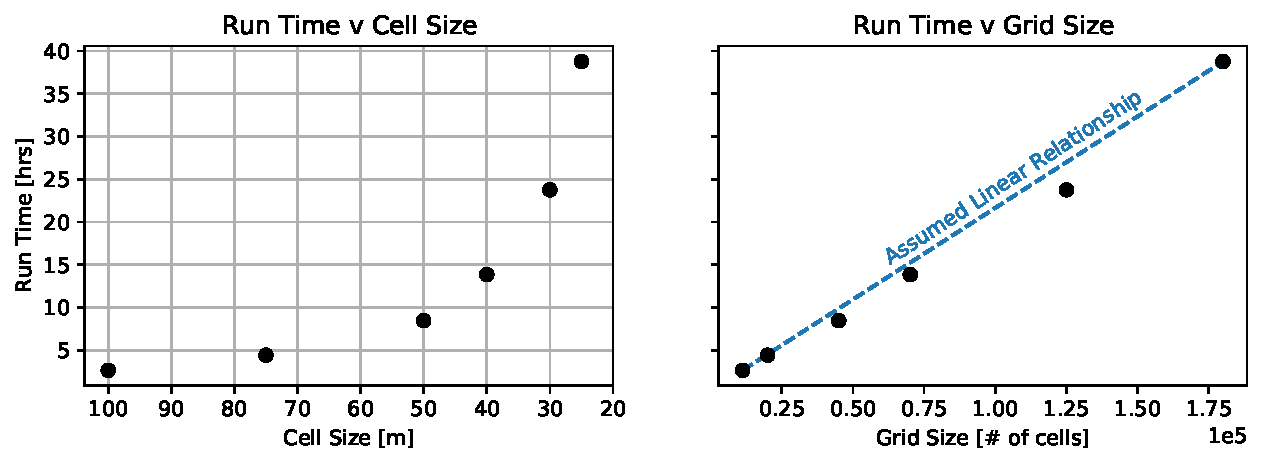
\includegraphics[width=\textwidth]{CellResRuntime/figs/RunTime_v_CellSize_naive.pdf}
	}	
	\caption{Results from the 6 runs generated by the YAML configuration file. \textit{Left:} Run time as a function of cell size. \textit{Right:} Run time as a function of the total number of cells in the domain.}
	\label{fig:res_v_runtime}
\end{figure}

\section{Conclusions}
There appears to be a linear relationship between the total number of grid cells in the domain and the runtime, and a nonlinear relationship between the cell resolution ($dx$) and runtime.
This finding is consistent, as the number of cells in a domain of fixed size scales inversely with the resolution of the individual cells ($dx$):

\begin{equation}
\text{\# cells} \sim \frac{1}{dx^2}
\end{equation}

Meaning that when the cell size is increased, the number of individual cells within the domain is reduced, and model runtime decreases. Conversely, when the cell resolution is increased, the number of cells increases, as does model runtime.

\clearpage
\bibliographystyle{plainnat}
\bibliography{bib/bib}
\label{chap:resruntime}

\chapter{Number of Parcels and Model Runtime}
\section{Background}
The number of parcels of water and sediment used for the weighted random walks influences the sensitivity of the model to extreme events \cite{Liang2015, Liang2015a}.
Therefore it is important to understand the relationship between the number of parcels used for a given model run and the runtime required.
This type of knowledge can help guide numerical experiment design. 

\section{Model Runs}
A set of 36 model runs, each with a different number of water parcels (\textit{Np\_{}water}) and a different number of sediment parcels (\textit{Np\_{}sed}) were conducted on a mini-domain.
The YAML below provides information about the domain and parameters used.\\

\noindent \texttt{YAML} configuration file: \vspace{-6pt}
\begin{boxedverbatim}
timesteps: 500
Length: 3000.0
Width: 5000.0
seed: 0
dx: 50.0
L0_meters: 50.0
N0_meters: 250.0
h0: 5.0
SLR: 36e-10  # small background SLR
save_dt: 250000

matrix:
  Np_sed:
    - 500
    - 1000
    - 1500
    - 2000
    - 2500
    - 3000
    
  Np_water:
    - 500
    - 1000
    - 1500
    - 2000
    - 2500
    - 3000
\end{boxedverbatim}

\section{Results}
The relationship between runtime, the number of water parcels, and the number of sediment parcels is plotted in 3-D space to inspect impact of the parcels on the time it takes for the model to run (Figure \ref{fig:np_v_runtime}).

\begin{sidewaysfigure}[!htbp]
	\makebox[\textwidth][c]{
	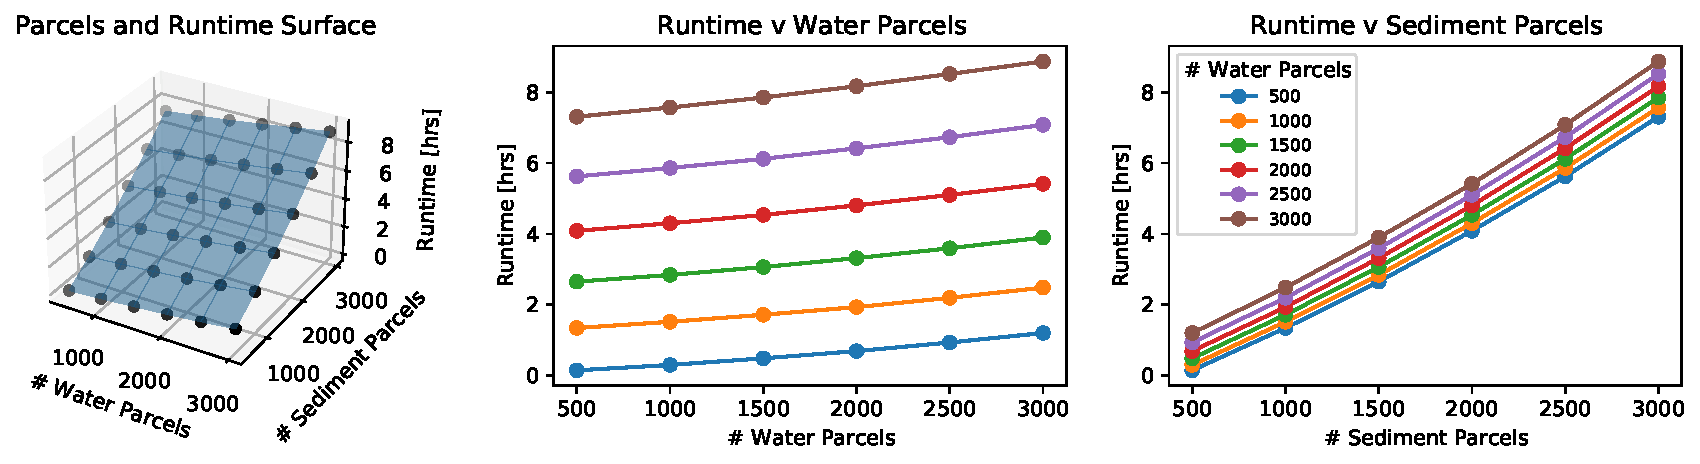
\includegraphics[width=\textwidth]{NumParcelsRuntime/figs/parcels_v_runtime.pdf}
	}	
	\caption{Results from the 36 runs. \textit{Left:} 3-D surface relating the number of water and sediment parcels to runtime. \textit{Center:} 2-D plot of runtime versus the number of water parcels, color indicates number of sediment parcels. \textit{Right:} Run time as a function of the number of sediment parcels, color indicates number of water parcels.}
	\label{fig:np_v_runtime}
\end{sidewaysfigure}

\section{Conclusions}
Water routing is computationally much cheaper than sediment routing as the cohort of parcels is routed in parallel.
This makes the increase in runtime for a greater number of water parcels much less dramatic than the increase in runtime when additional sediment parcels are used.
Increasing the number of sediment parcels can drastically raise the runtime required as these parcels are routed in serial, as each one modifies the topography as it moves through the domain.

\clearpage
\bibliographystyle{plainnat}
\bibliography{bib/bib}
\label{chap:npruntime}

\chapter{Model Variability}
\section{Background}
Understanding the intrinsic variability within the model is necessary when designing sets of experiments to ensure that the sample obtained is representative of generalized behavior.
Previous studies using the DeltaRCM methodology have run experiments in triplicate \cite{Liang2016a, Lauzon2018, Lauzon2019} as well as in sets of five \cite{Liang2016} to capture representative behavior under a given set of model conditions.
The underlying variability between model runs however, is not reported in these papers and remains an unknown (at the time of writing). 

\section{Model Runs}
\label{sec:standard_model_runs}
An ensemble of 30 model runs with different random seeds is generated.
These runs are at ``field-scale" using parameters similar to those from previous studies \cite{Liang2016, Liang2016a}.
The partial YAML file below provides information about the parameters used.\\

\noindent \texttt{YAML} configuration file: \vspace{-6pt}
\begin{boxedverbatim}
ensemble: 30
parallel: 3
Length: 7500
Width: 15000
timesteps: 5000
L0_meters: 150.0
N0_meters: 250.0
h0: 5.0
dx: 50
Np_water: 2000
Np_sed: 2000
save_dt: 250000
\end{boxedverbatim}

\section{Results}

Final topographies of all 30 deltas suggest that the overall shape and scale of these systems is similar (Figure \ref{fig:final_topos}). 
To quantify individual model behavior, land and channel maps are created by thresholding elevation and velocity data respectively.
Land is defined in locations where the elevation is at or above 0 m, and channels are pixels with velocity values in excess of 0.3 m/s (the threshold to mobilize sediment). 
Both of these thresholded arrays are bounded by a shoreline which is detected using morphological operators in a method similar to \citet{Geleynse2012}.
The method and its accuracy are not of primary interest here, but rather the differences between measurements from individual model runs. 

\begin{sidewaysfigure}[!htbp]
	\makebox[\textwidth][c]{
	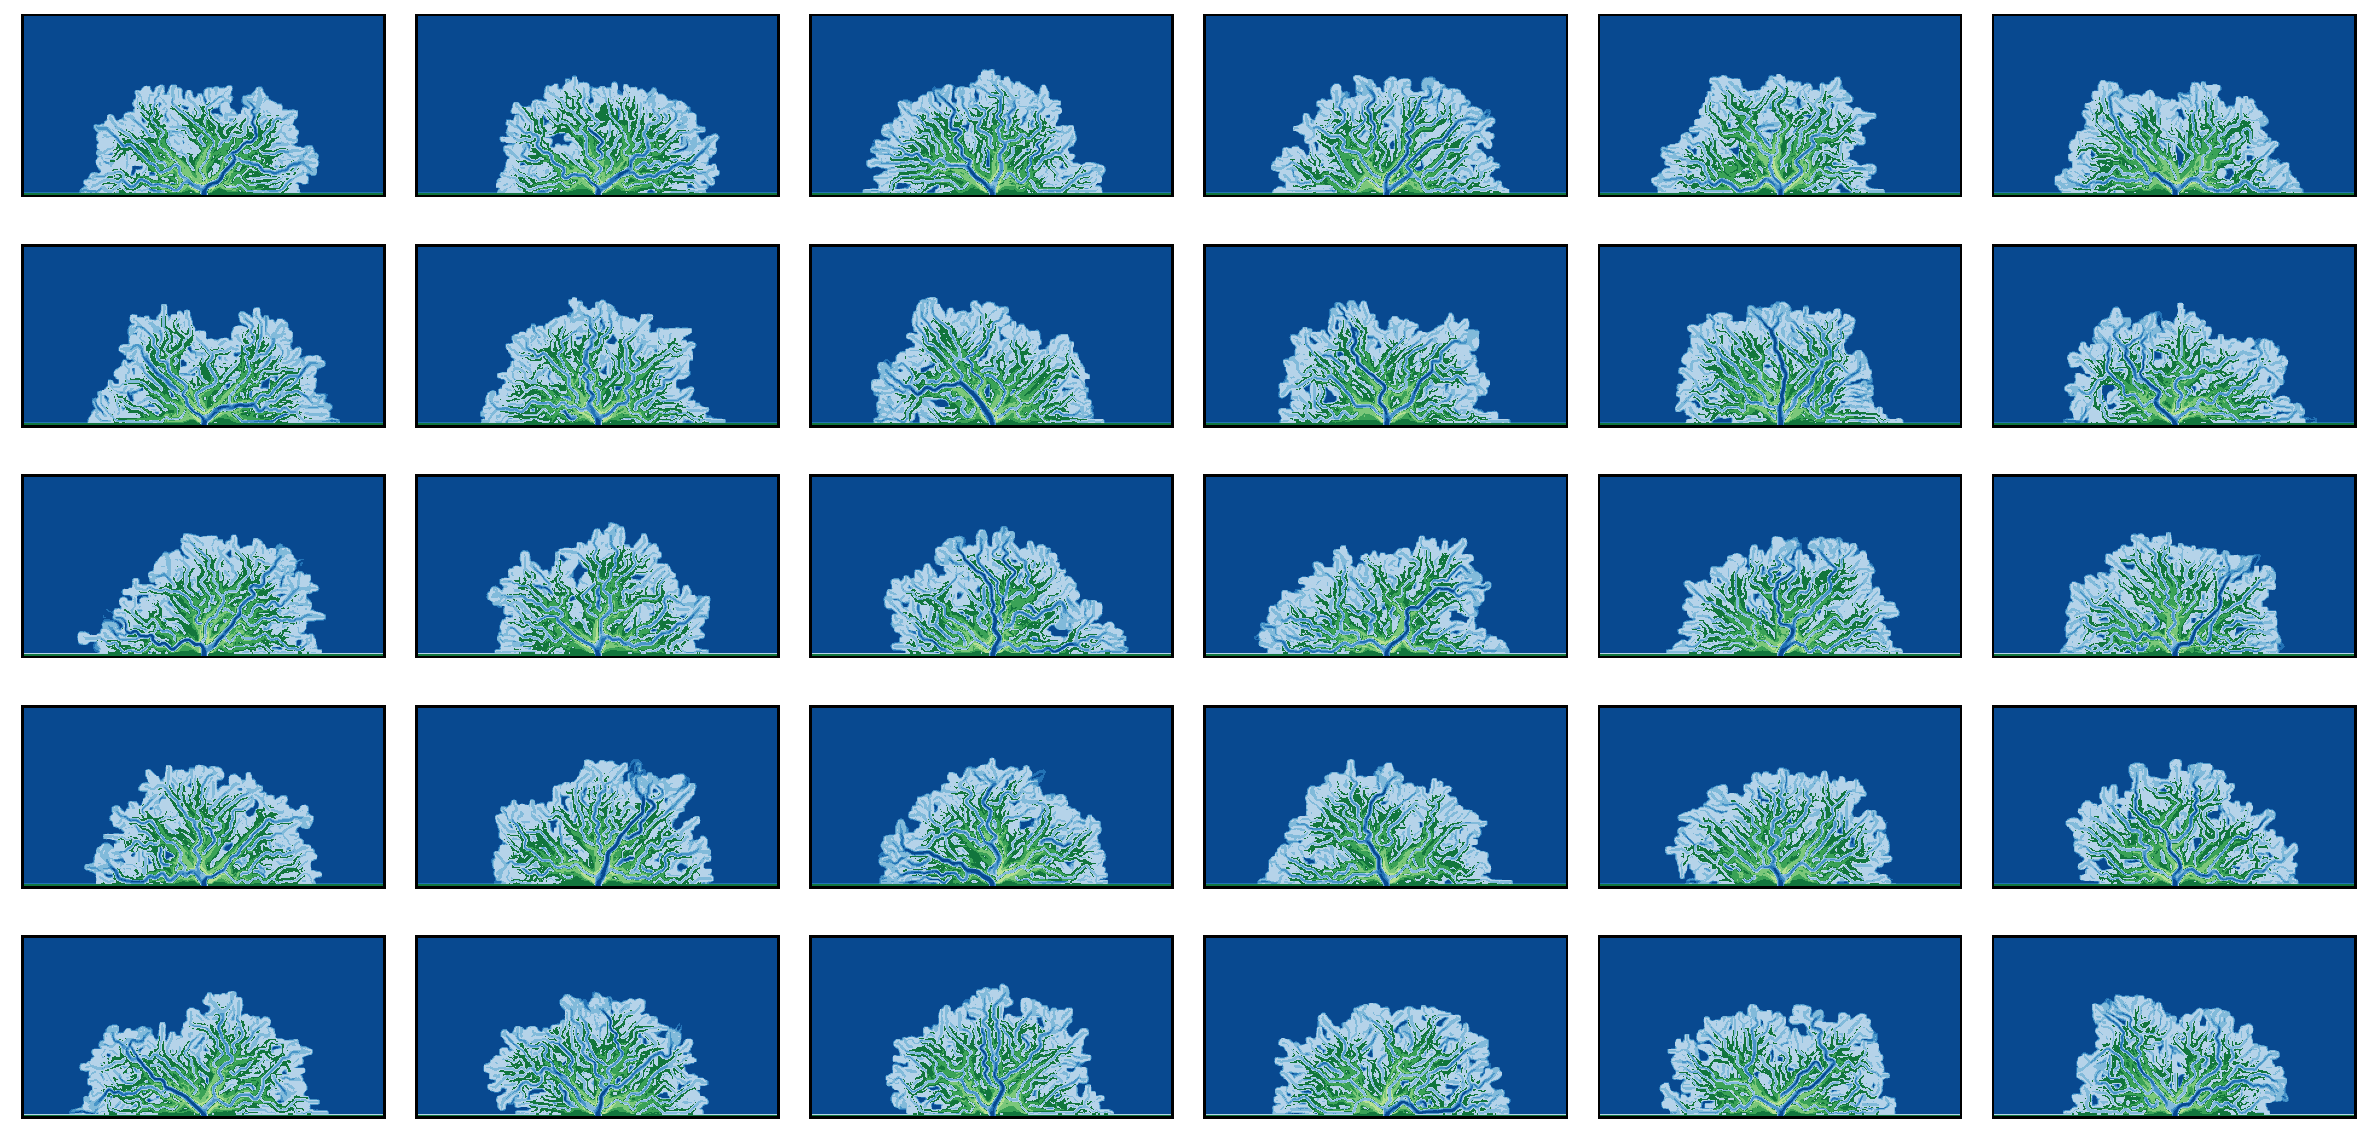
\includegraphics[width=\textwidth]{ModelVariability/figs/final_topos.pdf}
	}	
	\caption{Final topographies for the 30 ensemble runs.}
	\label{fig:final_topos}
\end{sidewaysfigure}

The three metrics measured are the land area, channel area, and fraction of land area that is channelized (channel fraction, Figure \ref{fig:surface_metrics}). 
Plots show individual replicate results in light gray, the ensemble mean in orange, and a blue envelope depicting the area within 1 standard deviation of the mean. 
Qualitatively there appears to be a fair amount of spread in these results.

\begin{sidewaysfigure}[!htbp]
	\makebox[\textwidth][c]{
	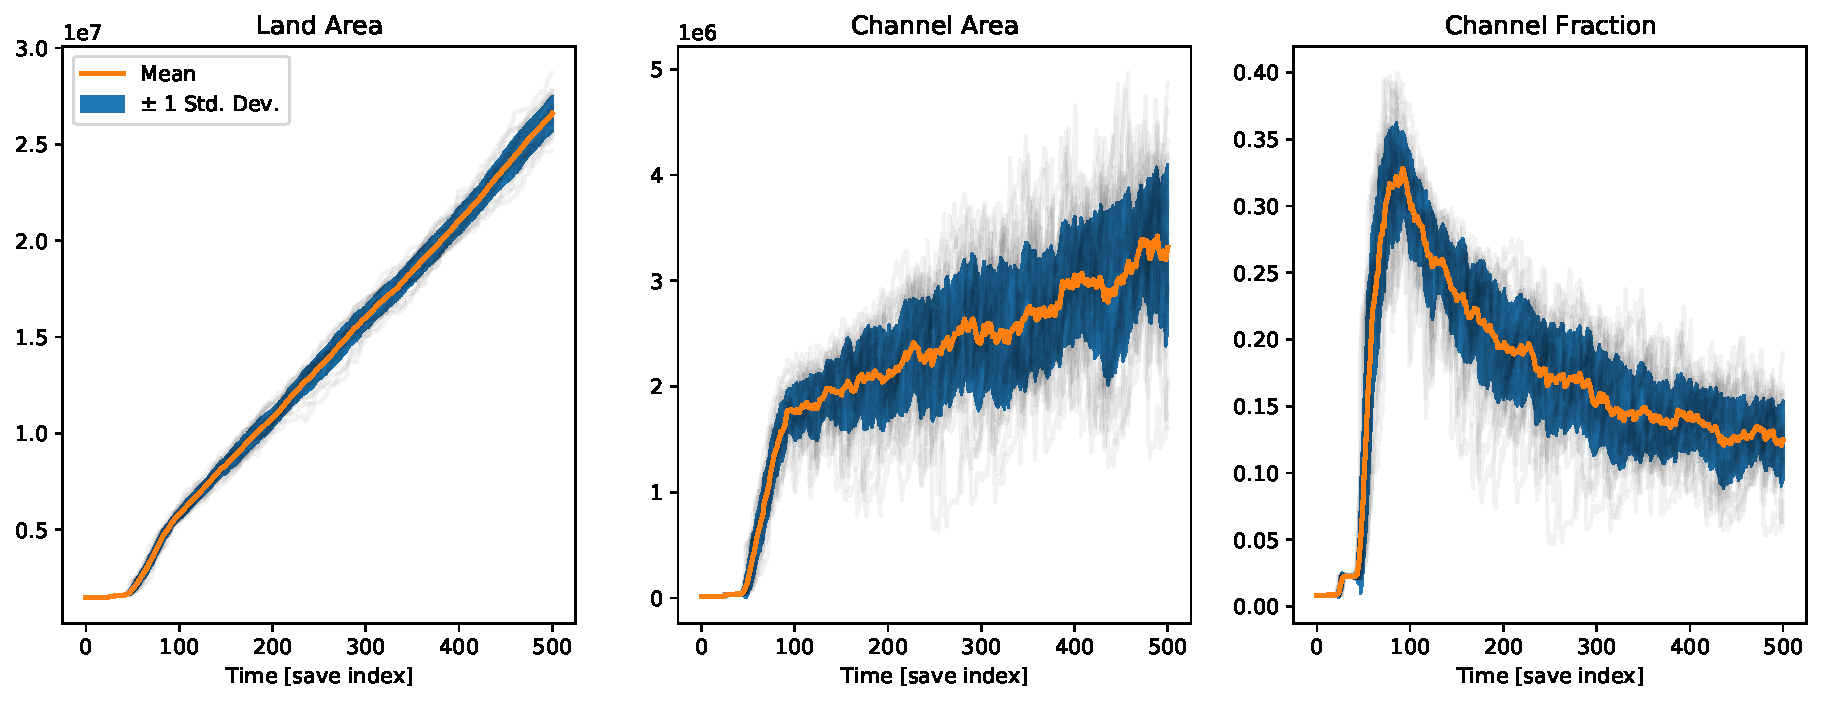
\includegraphics[width=\textwidth]{ModelVariability/figs/SurfaceTimeseries.pdf}
	}	
	\caption{Timeseries of 3 surface metrics: land area (left), channel area (center), and channel fraction, or the ratio of channel area to land area (right).}
	\label{fig:surface_metrics}
\end{sidewaysfigure}

To quantify this variability, a Monte Carlo approach is employed to estimate the probability of having a representative sample when using a smaller (less than 30) number of models.
The Monte Carlo method used works in the following way; to determine how representative a subset of $n$ models is, a random group of $n$ models from the full ensemble of 30 is chosen.
Next, a random point in time, $t_r$ is picked, and the land area, channel area, and channel fraction of the $n$ models is queried at time $t_r$, and a single average value for each metric is computed.
This average value is compared to the envelope plus/minus 1 standard deviation of the full ensemble mean (Figure \ref{fig:surface_metrics}), if the average value falls within the envelope, the Monte Carlo draw is deemed to be representative of the broader set.
The sampling process is repeated 1,000 times for each subset of $n$ models that is tested.
$n$ values between 1 and 10 are trialed as a reasonable range which includes the values of 3 and 5 used in previous studies.

For all three surface metrics evaluated, subsets of 3 or more models manage to fall within the `acceptable' envelope 90\% of the time or more. 
By the time the subset contains 7 models, this value has increased to 99\% (Table \ref{tab:tables}).
At 10 models, all three tables show nearly all draws fall within the envelope, suggesting that at least for these ``regular" or ``pseudo-default" parameters, no more than 10 models are needed to obtain a representative sample of model behavior for a given configuration.
Even subsets of fewer than 10 models are very likely to be representative of average behavior, anything above 3 appears to be a reasonable choice of replicates to use.

\begin{figure}[!htbp]
	\makebox[\textwidth][c]{
	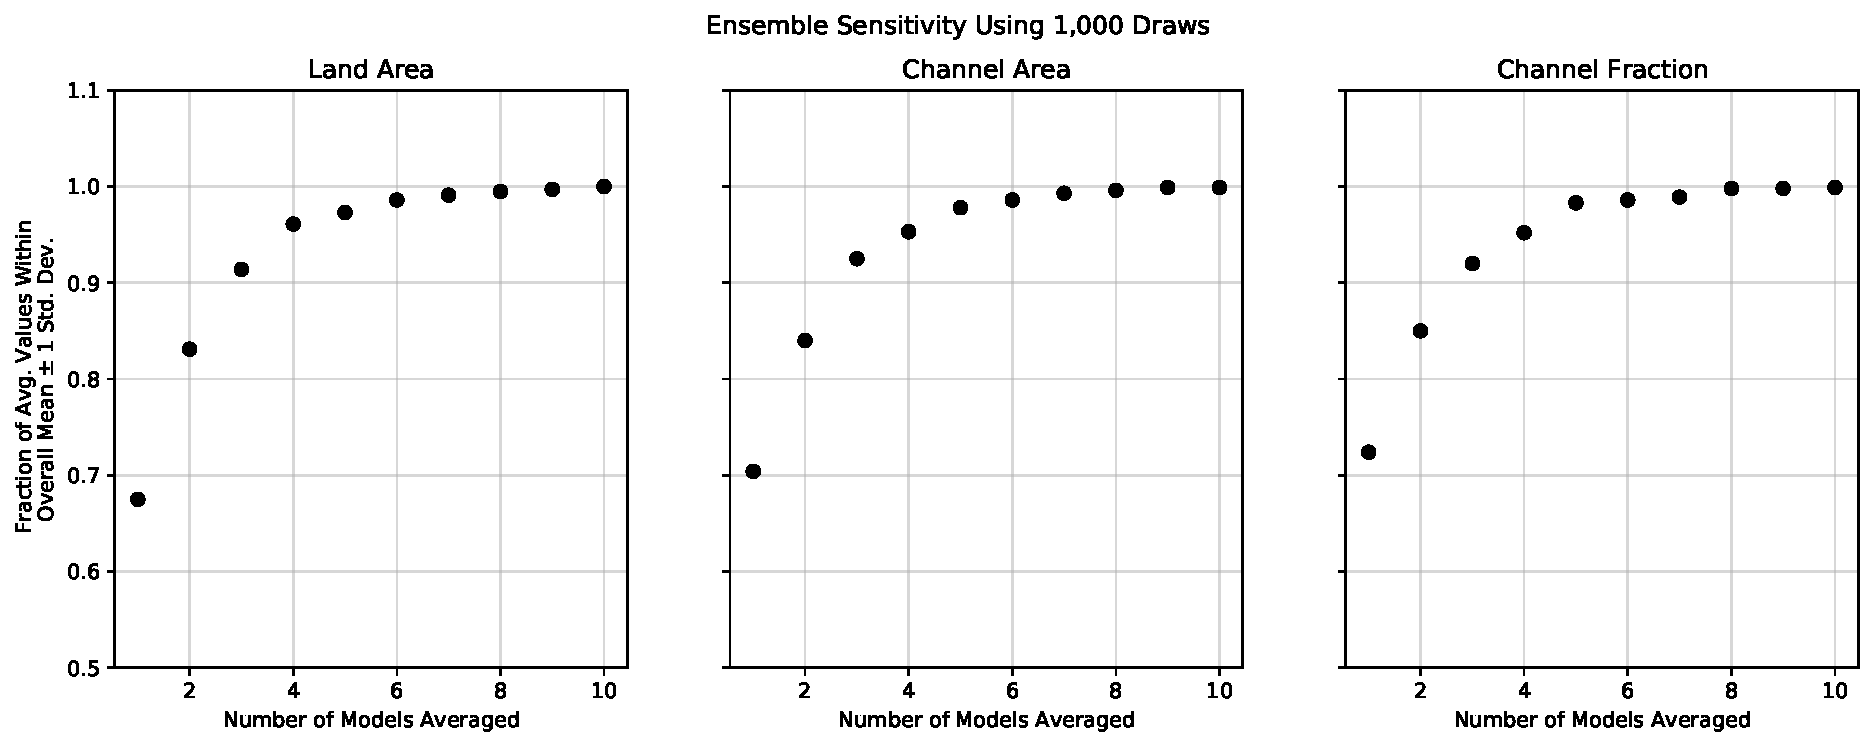
\includegraphics[width=\textwidth]{ModelVariability/figs/EnsembleSensitivity.pdf}
	}	
	\caption{Results of the sensitivity analysis for each of the surface metrics. Number of models in the Monte Carlo sampling along the x-axis and the fraction of average metric results within 1 standard deviation of the full dataset is on the y-axis.}
	\label{fig:MC_results}
\end{figure}

\begin{table}[!ht]
\begin{small}
\begin{tabular}{lcr}
\begin{minipage}[c]{0.3\linewidth}
\centering
\begin{tabular}{| l | r |}
\hline
\# Models & Fraction in Envelope \\
\hline
\hline
\csvreader[no head, late after line=\\\hline]
   {ModelVariability/tables/landsensitivity.csv}{}{\csvcoli & \csvcolii}
\end{tabular}
\label{tab:land}
\end{minipage}
&
\begin{minipage}[c]{0.3\linewidth}
\centering
\begin{tabular}{| l | r |}
\hline
\# Models & Fraction in Envelope \\
\hline
\hline
\csvreader[no head, late after line=\\\hline]
   {ModelVariability/tables/channelsensitivity.csv}{}{\csvcoli & \csvcolii}
\end{tabular}
\label{tab:land}
\end{minipage}
&
\begin{minipage}[c]{0.3\linewidth}
\centering
\begin{tabular}{| l | r |}
\hline
\# Models & Fraction in Envelope \\
\hline
\hline
\csvreader[no head, late after line=\\\hline]
   {ModelVariability/tables/fracsensitivity.csv}{}{\csvcoli & \csvcolii}
\end{tabular}
\label{tab:land}
\end{minipage}
\end{tabular}
\caption{Data from Figure \ref{fig:MC_results} presented in tabular form with the land area sensitivity on the left, channel area in the middle, and channel fraction on the right.}
\label{tab:tables}
\end{small}
\end{table}


\section{Conclusions}
While this is far from the most rigorous evaluation of intrinsic variability within the \textit{pyDeltaRCM} model, these results suggest that a minimum of 3 models should be run to characterize behavior representative of the domain and parameters. 
These results focus on just a few surface metrics, further tests should be conducted on the dynamics of the system as well as the stratigraphy produced, however given the number of studies previously conducted using 3 or 5 replicates, it is likely that unpublished sensitivity studies back up the findings reported here.

\clearpage
\bibliographystyle{plainnat}
\bibliography{bib/bib}

\chapter{Influence of Basin Depth, $hB$}
\section{Background}
Understanding the relationship between the depth of the basin, and properties about the resulting modeled delta can be helpful when trying to design numerical experiments.

\section{Model Runs}
Six model runs from Section \ref{sec:standard_model_runs} are used, and an addition 12 model runs in a 10m basin are conducted; 6 of which are run for 5,000 timesteps and the other 6 are run for 10,000 timesteps.
These runs are at ``field-scale" using parameters similar to those from previous studies \cite{Liang2016, Liang2016a}.
This is accomplished by varying the \textit{hB} YAML parameter in the model, the YAML is not included here for brevity, parameters are standard and match those of Section \ref{sec:standard_model_runs}.

\section{Results}
Example final topographies of the three model configurations are provided (Figure \ref{fig:bd_final_topos}), and examples of stratigraphic sections from the standard, 5m deep basin, as well as the 10,000 timestep 10m basin runs are shown (Figures \ref{fig:bd_dips}, \ref{fig:bd_radial}, \ref{fig:bd_horiz}). 

\begin{figure}[!ht]
	\makebox[\textwidth][c]{
	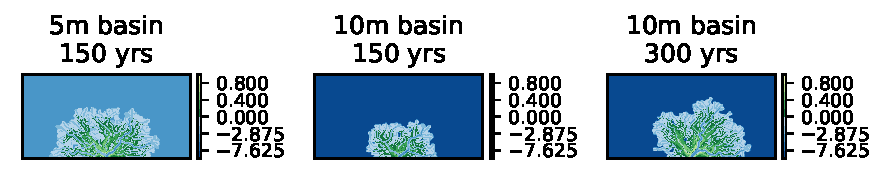
\includegraphics[width=\textwidth]{BasinDepth/figs/final_topos.pdf}
	}	
	\caption{Final topographies for the three scenarios considered.}
	\label{fig:bd_final_topos}
\end{figure}

\begin{figure}[!ht]
	\makebox[\textwidth][c]{
	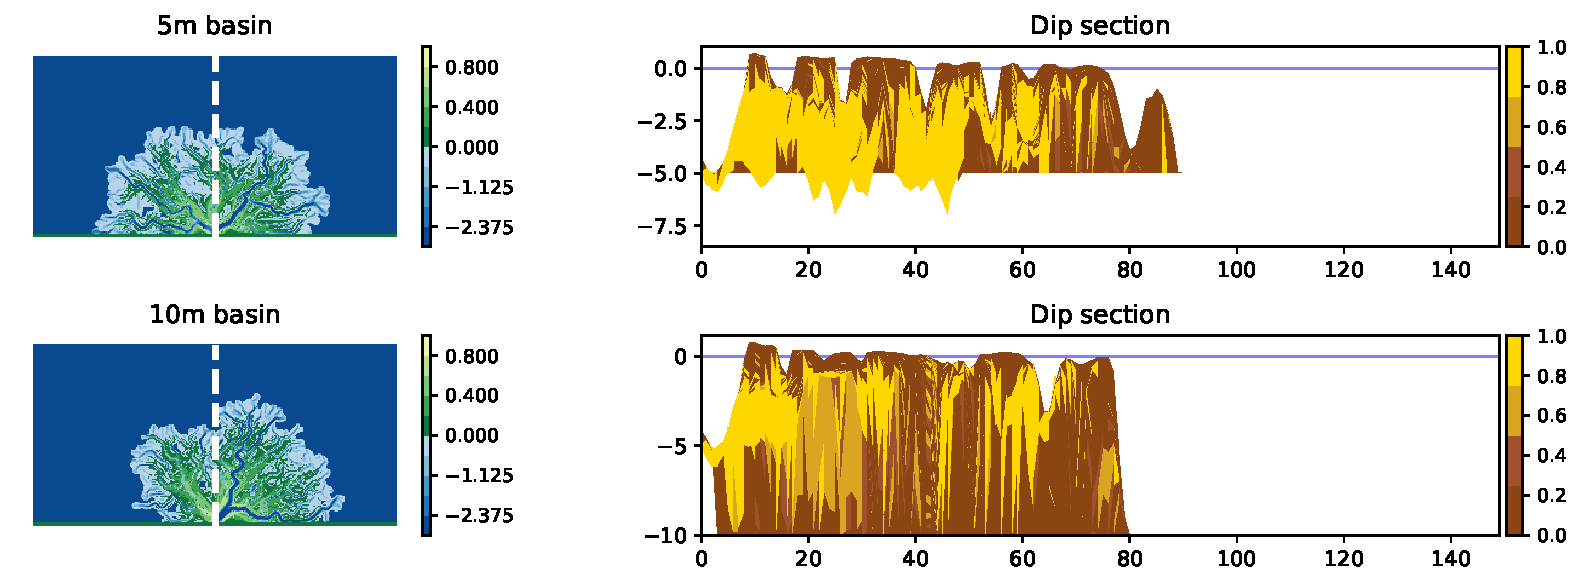
\includegraphics[width=\textwidth]{BasinDepth/figs/demo_dip_sections.pdf}
	}	
	\caption{Demo dip sections taken at the inlet location.}
	\label{fig:bd_dips}
\end{figure}

\begin{figure}[!ht]
	\makebox[\textwidth][c]{
	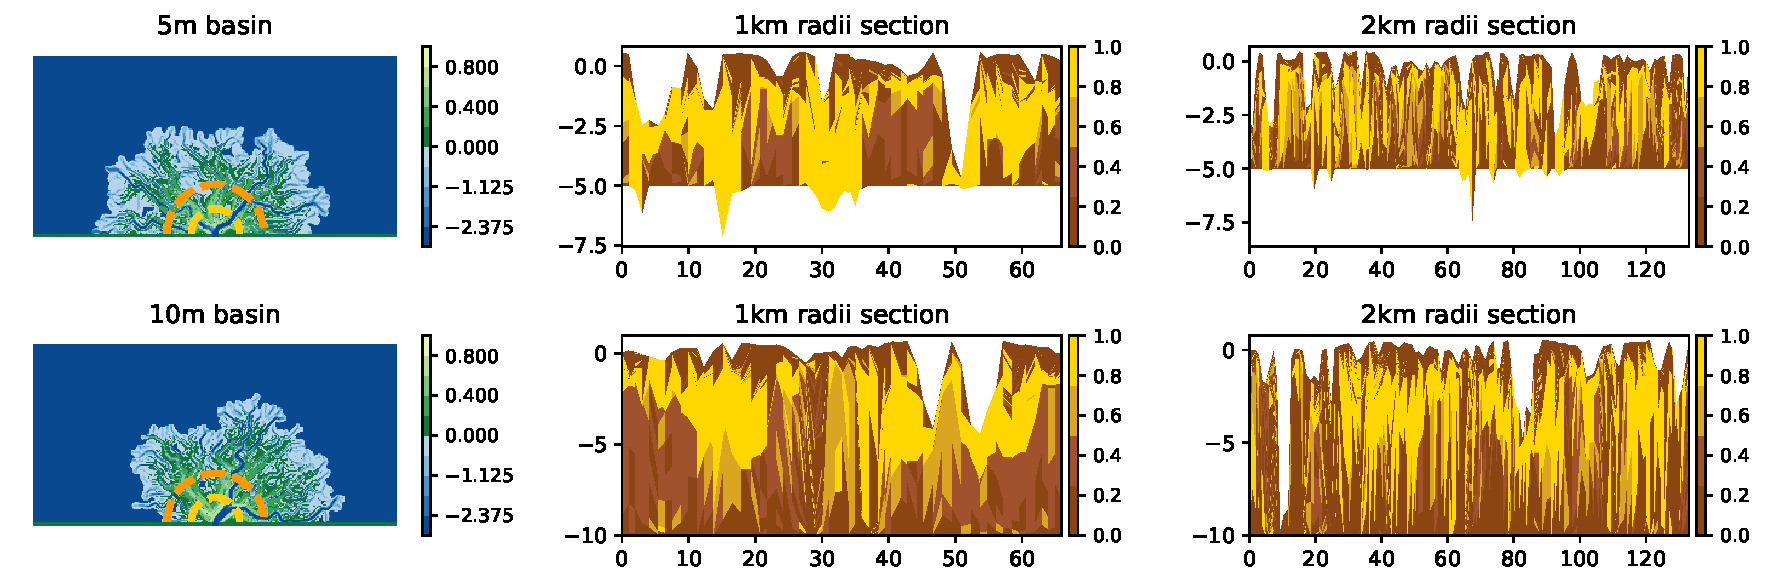
\includegraphics[width=\textwidth]{BasinDepth/figs/demo_radial_sections.pdf}
	}	
	\caption{Demo azimuthal sections taken with radii of 1 and 2km.}
	\label{fig:bd_radial}
\end{figure}

\begin{sidewaysfigure}[!ht]
	\makebox[\textwidth][c]{
	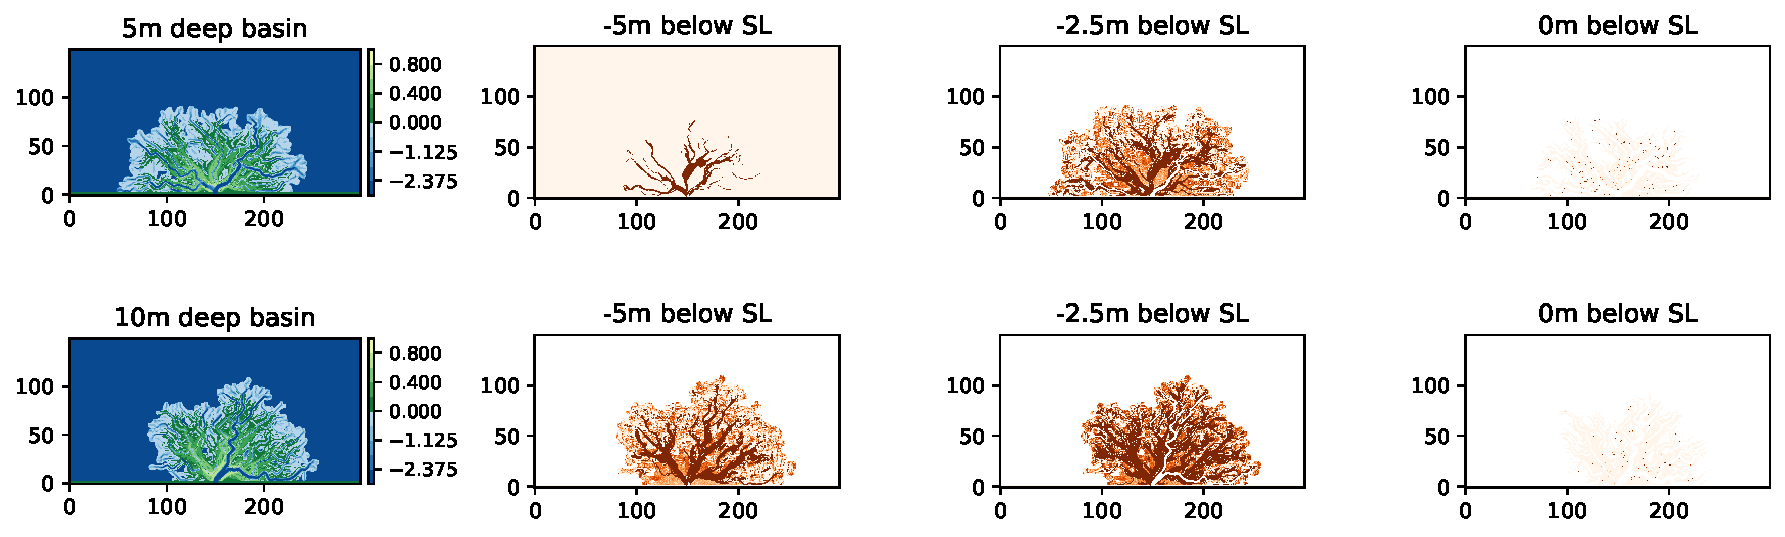
\includegraphics[width=\textwidth]{BasinDepth/figs/demo_horiz_sections.pdf}
	}	
	\caption{Demo horizontal slices of stratigraphy.}
	\label{fig:bd_horiz}
\end{sidewaysfigure}

Several metrics are calculated including the total land area of the modeled deltas (Figure \ref{fig:bd_land_area}), their channelized fractions (Figures \ref{fig:bd_chanfrac_timeseries} \& \ref{fig:bd_chanfrac_box}), and width-to-depth ratios of surface channels along several azimuthal transects with different radii (Figure \ref{fig:bd_wd}).

\begin{figure}[!ht]
	\makebox[\textwidth][c]{
	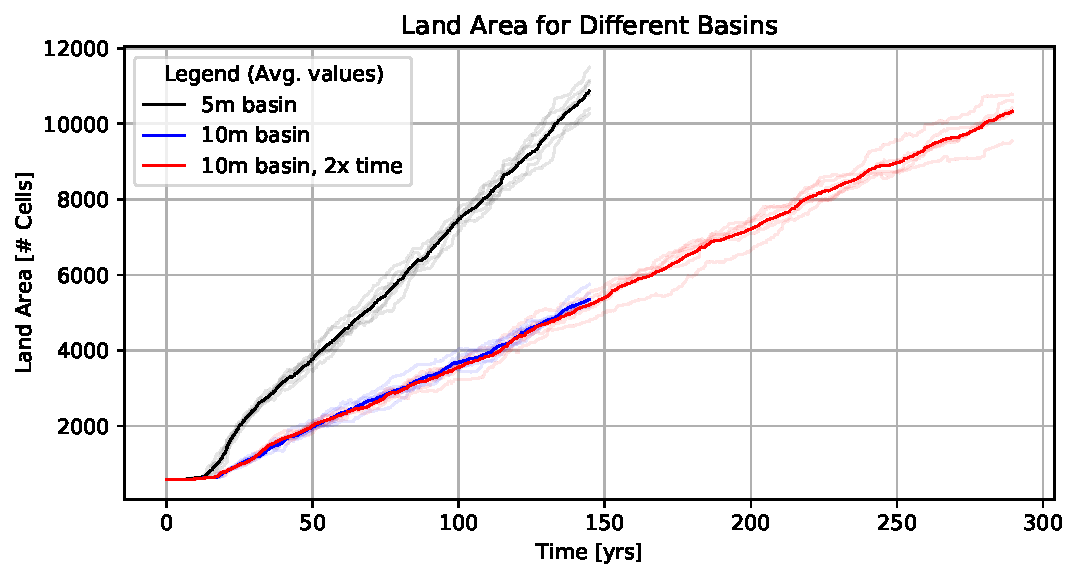
\includegraphics[width=\textwidth]{BasinDepth/figs/basin_land_timeseries.pdf}
	}	
	\caption{Land area timeseries, subaerial/subaqueous threshold value of 0m above sea level used.}
	\label{fig:bd_land_area}
\end{figure}

\begin{figure}[!ht]
	\makebox[\textwidth][c]{
	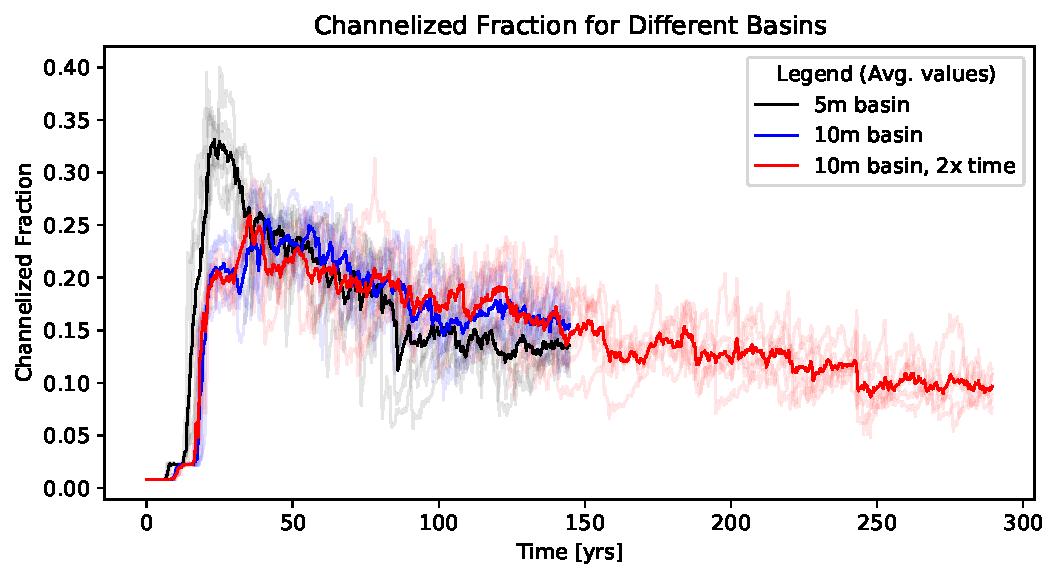
\includegraphics[width=\textwidth]{BasinDepth/figs/basin_chanfrac_timeseries.pdf}
	}	
	\caption{Timeseries of the fraction of the land area that is channelized.}
	\label{fig:bd_chanfrac_timeseries}
\end{figure}

\begin{figure}[!ht]
	\makebox[\textwidth][c]{
	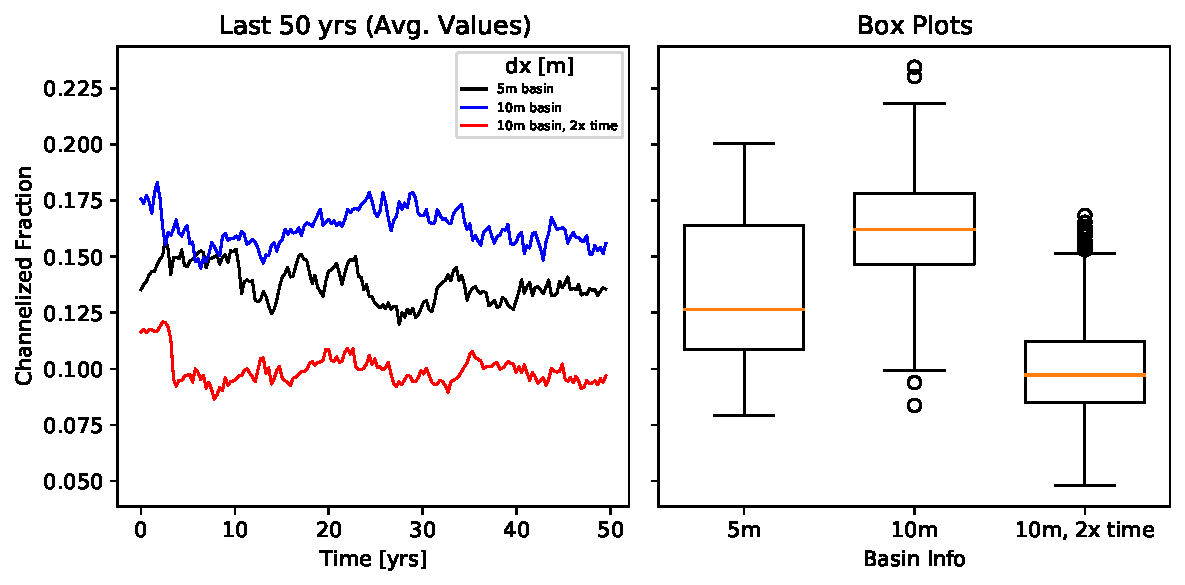
\includegraphics[width=\textwidth]{BasinDepth/figs/end_chanfrac_stationary.pdf}
	}	
	\caption{Average channel fraction from the final 50 years of each case (Left), and box plots of individual run channel fraction values over the final 50 years of each run split by basin scenario (Right).}
	\label{fig:bd_chanfrac_box}
\end{figure}

\begin{figure}[!ht]
	\makebox[\textwidth][c]{
	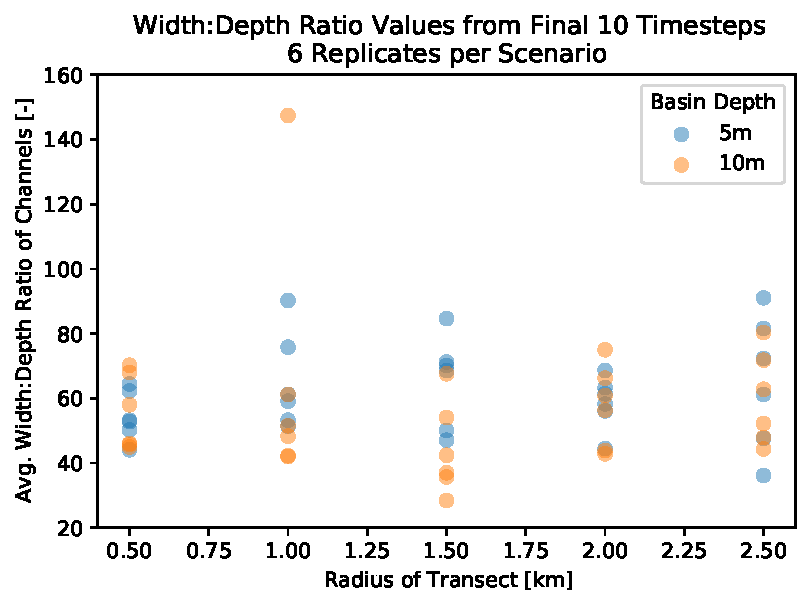
\includegraphics[width=\textwidth]{BasinDepth/figs/widthdepths_both.pdf}
	}	
	\caption{Average width-to-depth ratios from channels picked out along radial transects with different radii using the final 10 timesteps of the 5m deep basin scenario, and the 10m basin depth, 10,000 timestep scenario.}
	\label{fig:bd_wd}
\end{figure}

\section{Conclusions}
Beyond slowing the lateral growth of the system due to the deeper basin, there don't appear to be real differences between the two.
Both the width-to-depth ratios of the surface channels and the proportion of the subaerial surface that was channelized appeared to be similar (Figures \ref{fig:bd_wd} \& \ref{fig:bd_chanfrac_timeseries}).
When qualitatively looking at the stratigraphy, there is not much to comment on besides the obvious preservation of $\sim$ 10m of stratigraphy in the 10m basin, and $\sim$ 5m in the shallower 5m basin.

\clearpage
\bibliographystyle{plainnat}
\bibliography{bib/bib}

\chapter{Impact of Alpha value, $\alpha$}
\section{Background}
The alpha parameter ($\alpha$) is a topographic diffusion coefficient, and influences both cross-slope sediment flux and bank erodibility.
While detailed investigation into a similar parameter in the Delft3D morphodynamic model has been conducted \citep{Baar2019}, a similar analysis has not been conducted using DeltaRCM or pyDeltaRCM.
The reduced complexity approach in the DeltaRCM model is inspired by the Bagnold-Ikeda formulation in \citet{Garcia2008}, \citep{Liang2015a}.

\section{Model Runs}
To test the influence of the $\alpha$ YAML parameter, runs with the following parameters were conducted in triplicate with alpha values of $\alpha = 0.01, 0.05, 0.1, 0.5, 1.0, 5.0, 10.0$.
The YAML below provides information about the parameter set used.\\

\noindent \texttt{YAML} configuration file: \vspace{-6pt}
\begin{boxedverbatim}
Length: 7500
Width: 15000
timesteps: 5000
L0_meters: 150.0
N0_meters: 250.0
dx: 50.0
h0: 5.0
Np_water: 2000
Np_sed: 2000
save_dt: 250000
\end{boxedverbatim}

\section{Results}
The influence of the alpha parameter can be seen when looking at the final topographies generated by the various models (Figure \ref{fig:alpha_topos}).
The effect diffusion of the topography has on the channels can be seen more clearly in Figure \ref{fig:alpha_transect} which provides a visualization of an azimuthal transect sliced through the system.
Finally, the width-to-depth ratios of the surface channels are also impacted by the different degrees of topographic diffusion (Figure \ref{fig:alpha_wd}).

\begin{sidewaysfigure}[!ht]
	\makebox[\textwidth][c]{
	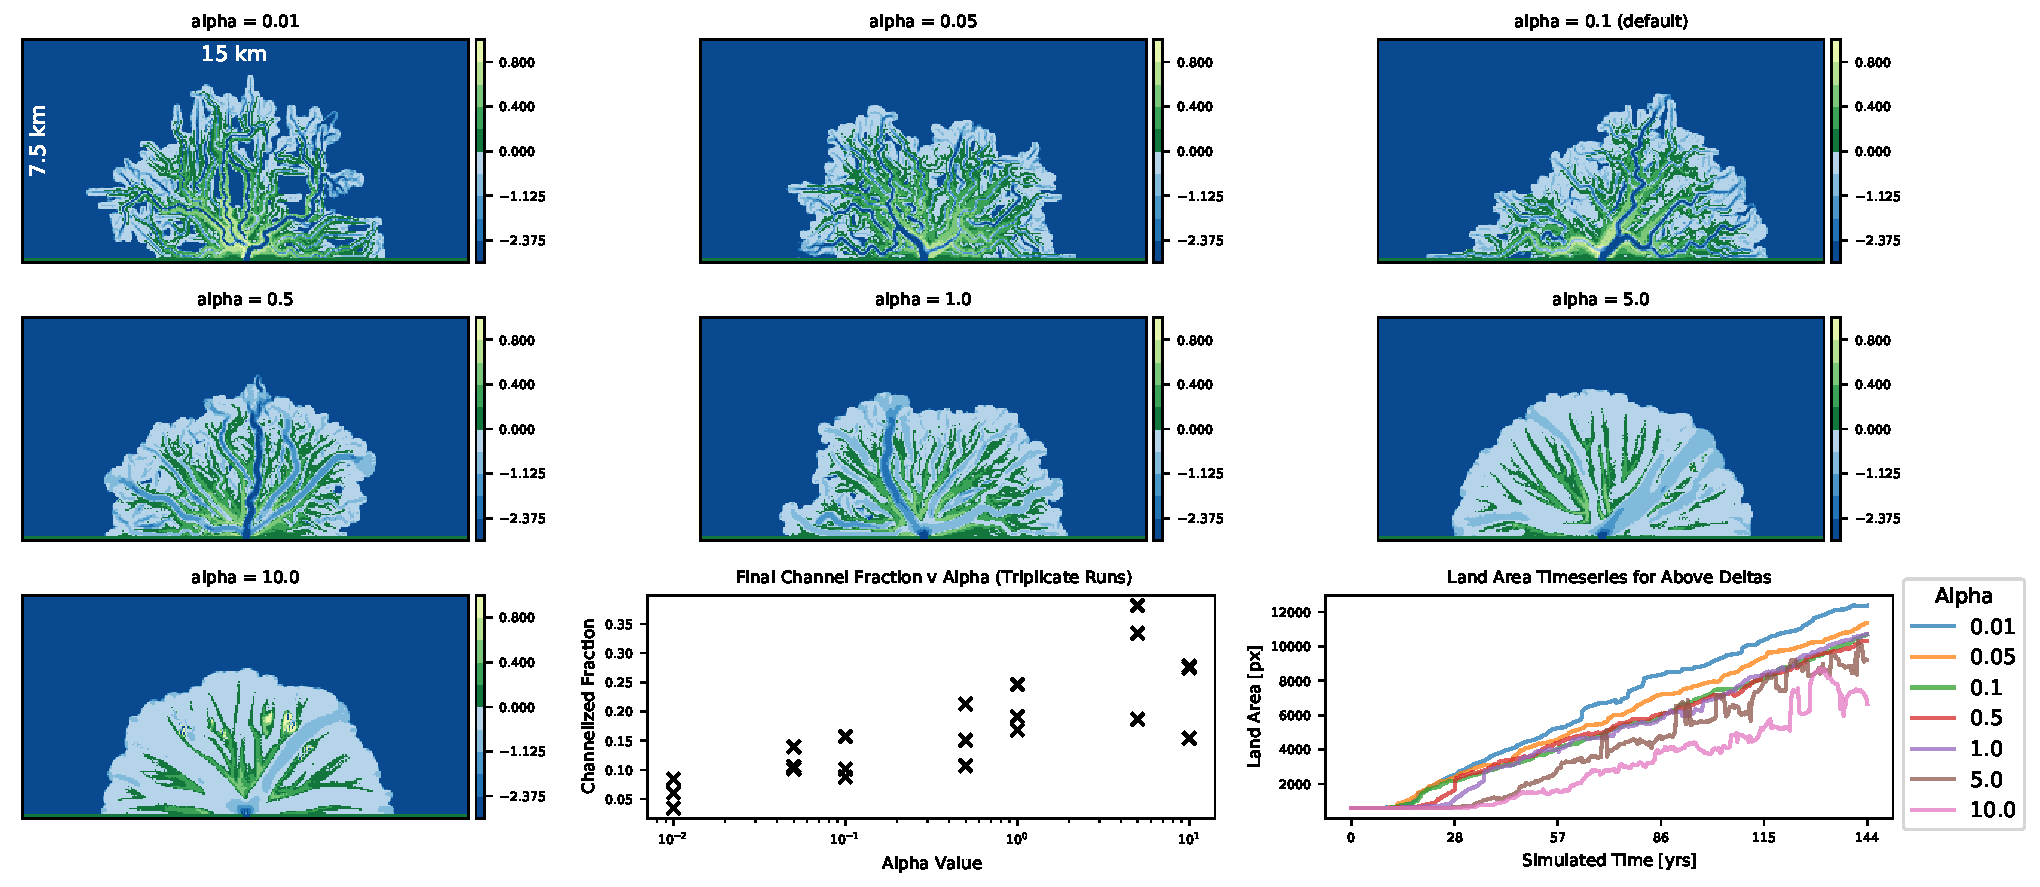
\includegraphics[width=\textwidth]{AlphaImpact/figs/alpha_results.pdf}
	}	
	\caption{Examples of the final topographies obtained for different values. \textit{Bottom, center:} Channelized fractions at the end of each model run as a function of the alpha parameter. \textit{Bottom, right:} Land area timeseries for one model per alpha parameter.}
	\label{fig:alpha_topos}
\end{sidewaysfigure}

\begin{sidewaysfigure}[!ht]
	\makebox[\textwidth][c]{
	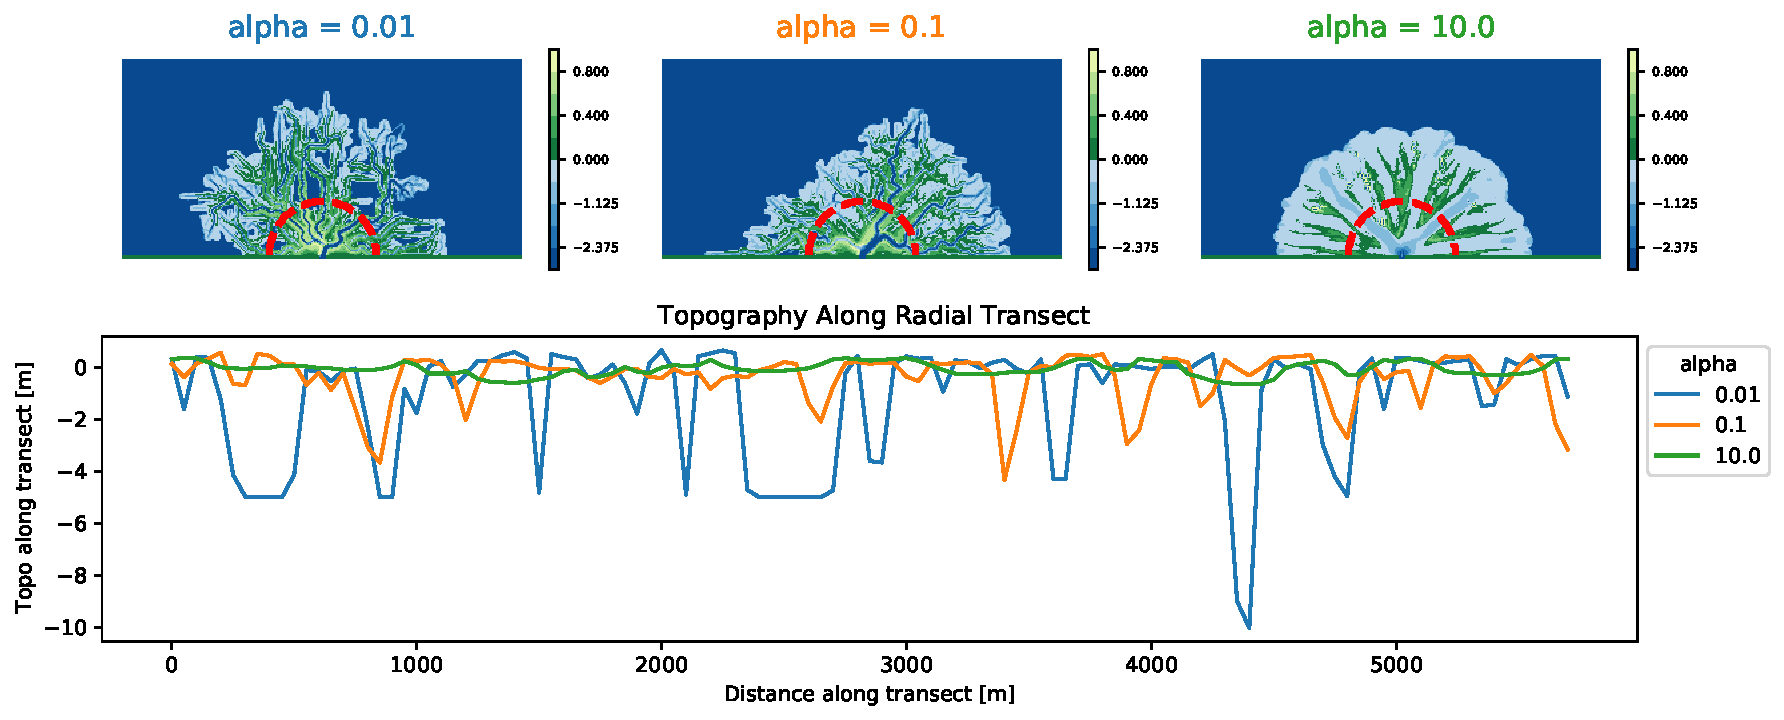
\includegraphics[width=\textwidth]{AlphaImpact/figs/topotransect_alpha.pdf}
	}	
	\caption{Topography transects for the lowest, default, and highest alpha values tested to visualize the impact of topographic diffusion on the channel geometries.}
	\label{fig:alpha_transect}
\end{sidewaysfigure}

\begin{figure}[!ht]
	\makebox[\textwidth][c]{
	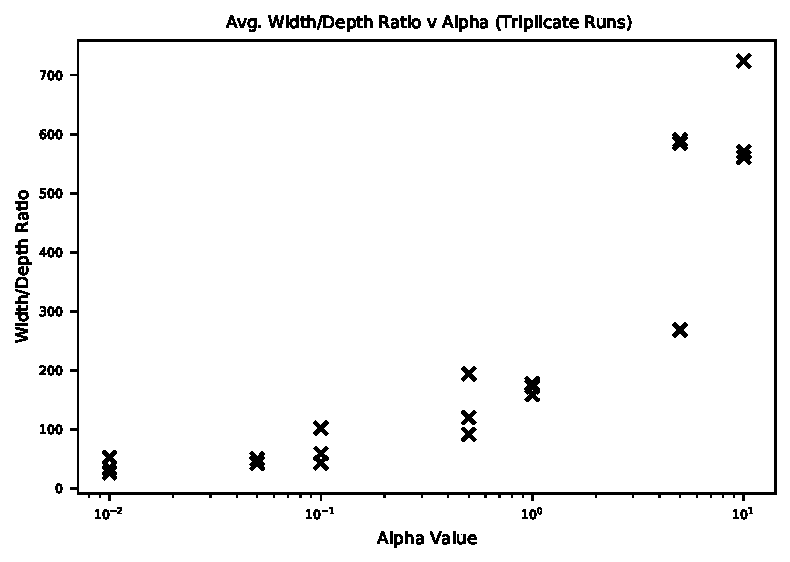
\includegraphics[width=\textwidth]{AlphaImpact/figs/widthdepth_alpha.pdf}
	}	
	\caption{Plot of average width-to-depth ratios as a function of the different alpha values. Width-to-depth ratios are calculated along the azimuthal transects visualized in Figure \ref{fig:alpha_transect}.}
	\label{fig:alpha_wd}
\end{figure}

\section{Conclusions}
The alpha parameter clearly influences the simulated deltas.
Values close to the default value of 0.1 appear to have only slight impacts on the topography and channel properties.
Once the alpha parameter deviates more significantly from its default, significant impacts to the visual appearance of the deltas as well as properties related to the channels occur.
These results appear consistent with those observed in \citet{Baar2019} when a similar property was tested using in Delft3D.

\clearpage
\bibliographystyle{plainnat}
\bibliography{bib/bib}

\chapter{Impact of Beta value, $\beta$}
\section{Background}
The beta exponent ($\beta$) dictates the transport capacity ($q_{s\_{}cap}$) of individual sand parcels as
\begin{equation}
	q_{s\_{}cap} = q_{s0} \frac{u_{loc}^{\beta}}{u_{0}^{\beta}},
\end{equation}
where $q_{s0}$ is the upstream sand flux input divided by the inlet channel width.
This scaling is based on the Meyer-Peter and Muller \citep{meyer1948formulas} formulation and is a nonlinear function of local flow velocity.
Therefore, by changing the value of $\beta$, the transport behavior for sand parcels can be altered for the given simulation.

\section{Model Runs}
To test the influence of the $\beta$ YAML parameter, runs with the following parameters were conducted in triplicate with beta values of $\beta = 1, 2, 3, 4, 5, 10, 15$.
The YAML below provides information about the parameter set used.\\

\noindent \texttt{YAML} configuration file: \vspace{-6pt}
\begin{boxedverbatim}
Length: 7500
Width: 15000
timesteps: 5000
L0_meters: 150.0
N0_meters: 250.0
dx: 50.0
h0: 5.0
Np_water: 2000
Np_sed: 2000
save_dt: 250000
\end{boxedverbatim}

\section{Results}
The influence of the beta parameter can be seen when looking at the final topographies generated by the various models (Figure \ref{fig:beta_topos}).

\begin{sidewaysfigure}[!ht]
	\makebox[\textwidth][c]{
	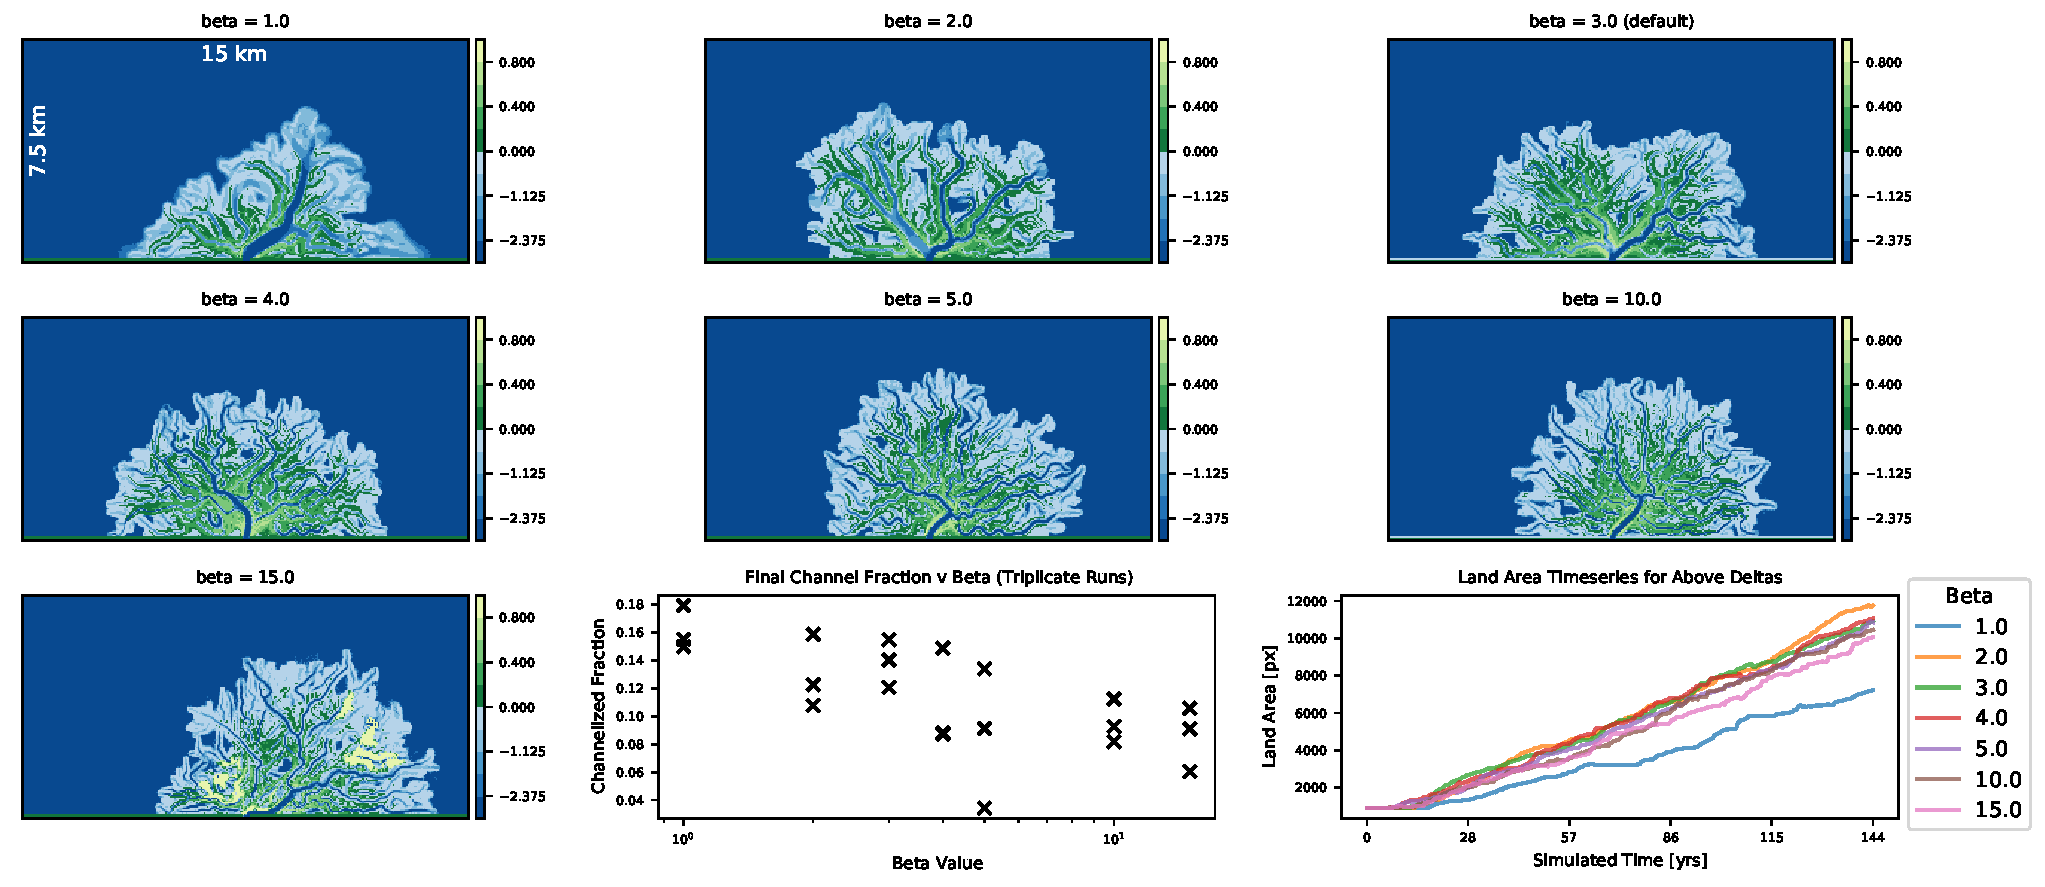
\includegraphics[width=\textwidth]{BetaImpact/figs/beta_results.pdf}
	}	
	\caption{Examples of the final topographies obtained for different values of $\beta$. \textit{Bottom, center:} Channelized fractions at the end of each model run as a function of the beta parameter. \textit{Bottom, right:} Land area timeseries for one model per beta parameter.}
	\label{fig:beta_topos}
\end{sidewaysfigure}

\begin{sidewaysfigure}[!ht]
	\makebox[\textwidth][c]{
	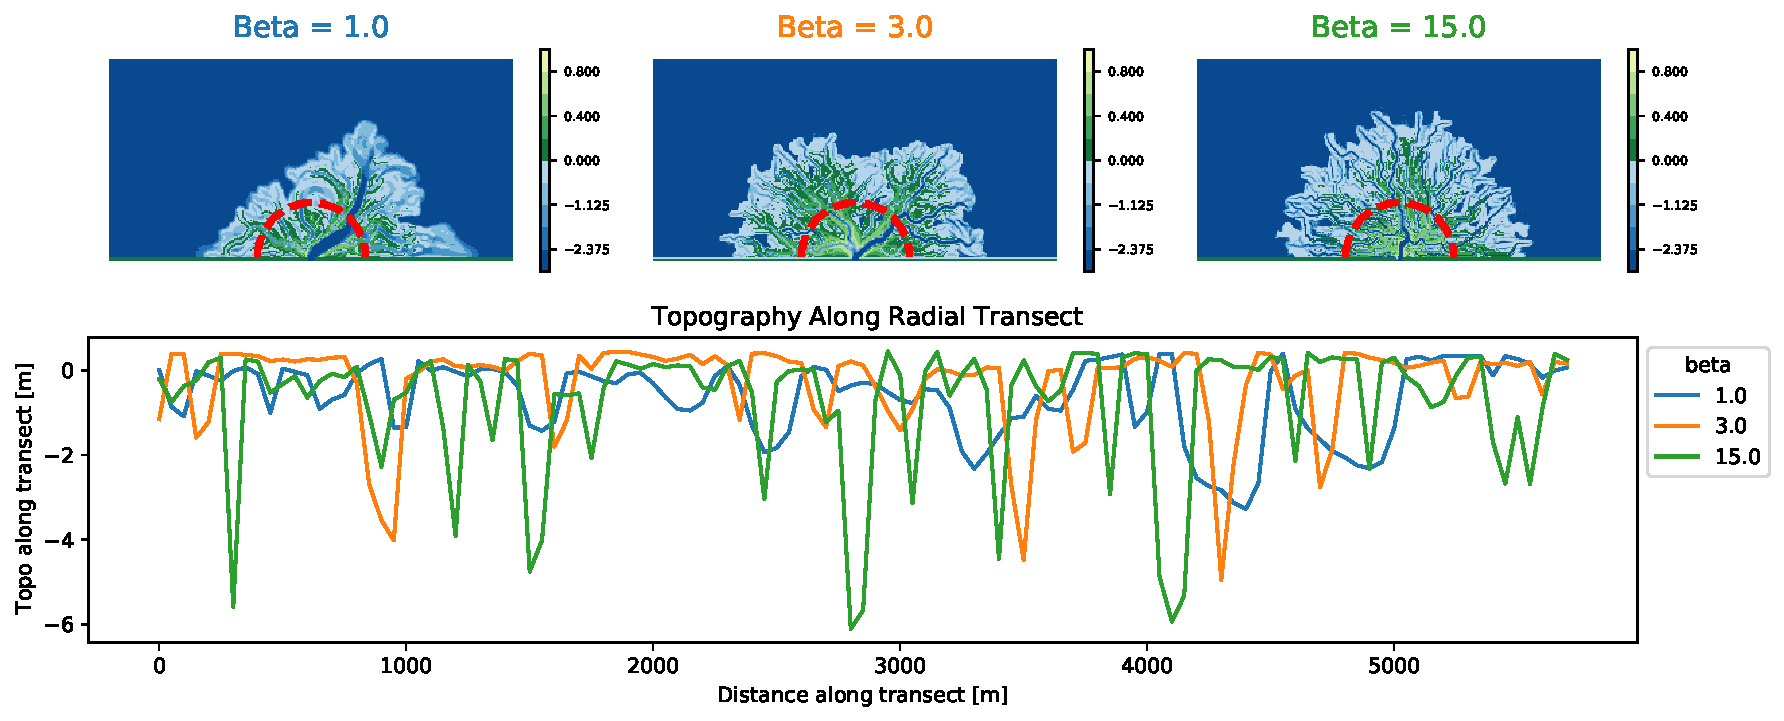
\includegraphics[width=\textwidth]{BetaImpact/figs/topotransect_beta.pdf}
	}	
	\caption{Topography transects for the lowest, default, and highest beta values tested to visualize the impact of topographic diffusion on the channel geometries.}
	\label{fig:beta_transect}
\end{sidewaysfigure}

\begin{figure}[!ht]
	\makebox[\textwidth][c]{
	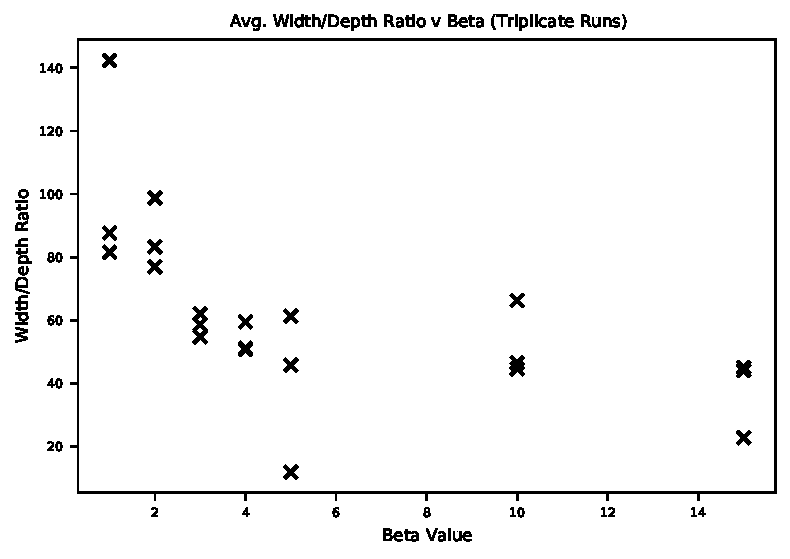
\includegraphics[width=\textwidth]{BetaImpact/figs/widthdepth_beta.pdf}
	}	
	\caption{Plot of average width-to-depth ratios as a function of the different beta values. Width-to-depth ratios are calculated along the azimuthal transects visualized in Figure \ref{fig:beta_transect}.}
	\label{fig:beta_wd}
\end{figure}

\section{Conclusions}
The beta parameter clearly influences the simulated deltas.
When $\beta$ greatly exceeds the default value of 3.0, then the model can become unstable.
Results here for $\beta$ values of 15 resulted in portions of the delta having unrealistically high elevations on the order of 1,000 meters above sea level.
Similarly when the value of beta becomes too small, the result can be unrealistic.
This is evident in the runs conducted with beta values of 1.0 in which the capacity of the sand parcels must be near-zero, and therefore the system is far to diffusive.

\clearpage
\bibliographystyle{plainnat}
\bibliography{bib/bib}

\chapter{Cell Resolution Impact on Model Results}
\section{Background}
Understanding the impact cell resolution ($dx$) has on model behavior, delta morphology, dynamics, and stratigraphy is important, as model resolution influences the model's runtime (Chapter \ref{chap:resruntime}).

\section{Model Runs}
A set of 4 cell resolution values are used and model runs are conducted in triplicate.
These runs are at ``field-scale" using parameters similar to those from previous studies \cite{Liang2016, Liang2016a}.
The YAML below provides information about the parameter set used.\\

\noindent \texttt{YAML} configuration file: \vspace{-6pt}
\begin{boxedverbatim}
ensemble: 3
Length: 7500
Width: 15000
timesteps: 5000
L0_meters: 150.0
N0_meters: 300.0
SLR: 36e-10  # slight maybe 3 mm/yr SLR
save_dt: 300000  # every 10 timesteps (dt = 30000)

matrix:
  dx:
    - 30.0
    - 50.0
    - 75.0
    - 100.0
\end{boxedverbatim}

\section{Results}
Final topographies, as well as corresponding channel maps are visualized (Figures \ref{fig:res_finaltopo} \& \ref{fig:res_chanmap}).
Channel fraction timeseries for all runs is computed (Figure \ref{fig:res_chanfrac_timeseries}), as is the channelized fraction over the final 50 years for each run for which box-plots for each cell resolution are created (Figure \ref{fig:res_chanfrac}).
Channel widths and depths are calculated along azimuthal transects based on the location of surface channels (from Figure \ref{fig:res_chanmap}), using the final topography (from Figure \ref{fig:res_finaltopo}), the average width and depth values are plotted (Figure \ref{fig:res_depth_v_width}), as are the width-to-depth ratios as a function of model cell resolution (Figure \ref{fig:res_wd}).

\begin{figure}[!ht]
	\makebox[\textwidth][c]{
	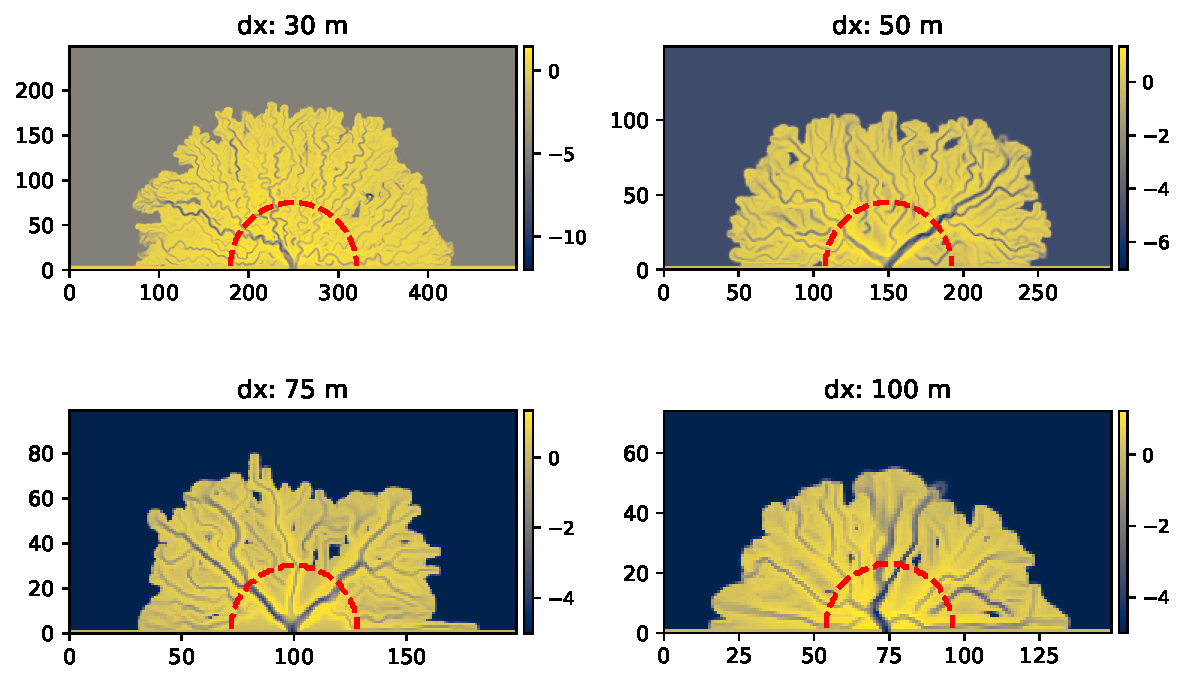
\includegraphics[width=\textwidth]{CellResAnalysis/figs/circ_planview.pdf}
	}	
	\caption{Final topography for different cell resolutions with the location of the azimuthal transect used for channel width and depth measurements shown as a dashed red line.}
	\label{fig:res_finaltopo}
\end{figure}

\begin{figure}[!ht]
	\makebox[\textwidth][c]{
	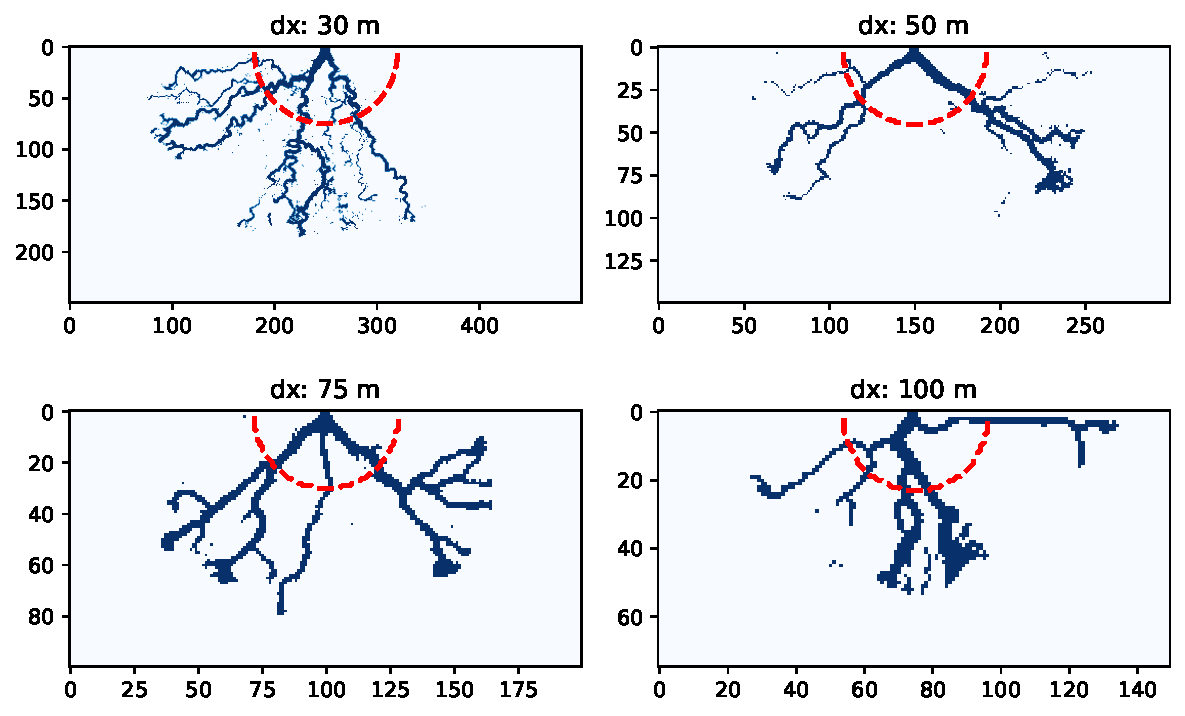
\includegraphics[width=\textwidth]{CellResAnalysis/figs/circular_planview.pdf}
	}	
	\caption{Binary surface channel maps at the final timestep for the different cell resolutions, surface channels identified as cells with water velocities exceeding 0.3 m/s.}
	\label{fig:res_chanmap}
\end{figure}

\begin{figure}[!ht]
	\makebox[\textwidth][c]{
	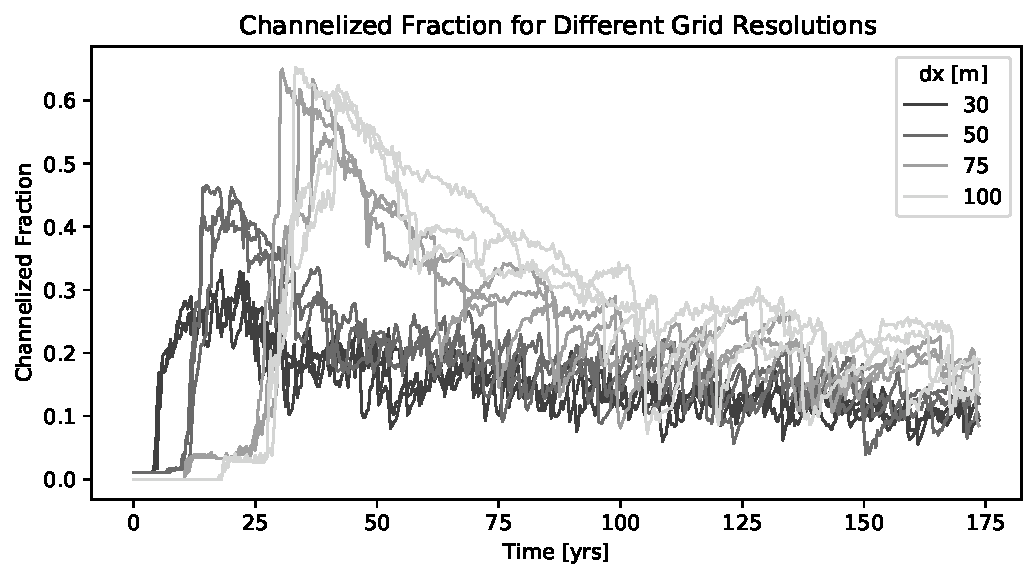
\includegraphics[width=\textwidth]{CellResAnalysis/figs/chanfrac_timeseries.pdf}
	}	
	\caption{Timeseries of channelized fraction values for all of the model runs.}
	\label{fig:res_chanfrac_timeseries}
\end{figure}

\begin{figure}[!ht]
	\makebox[\textwidth][c]{
	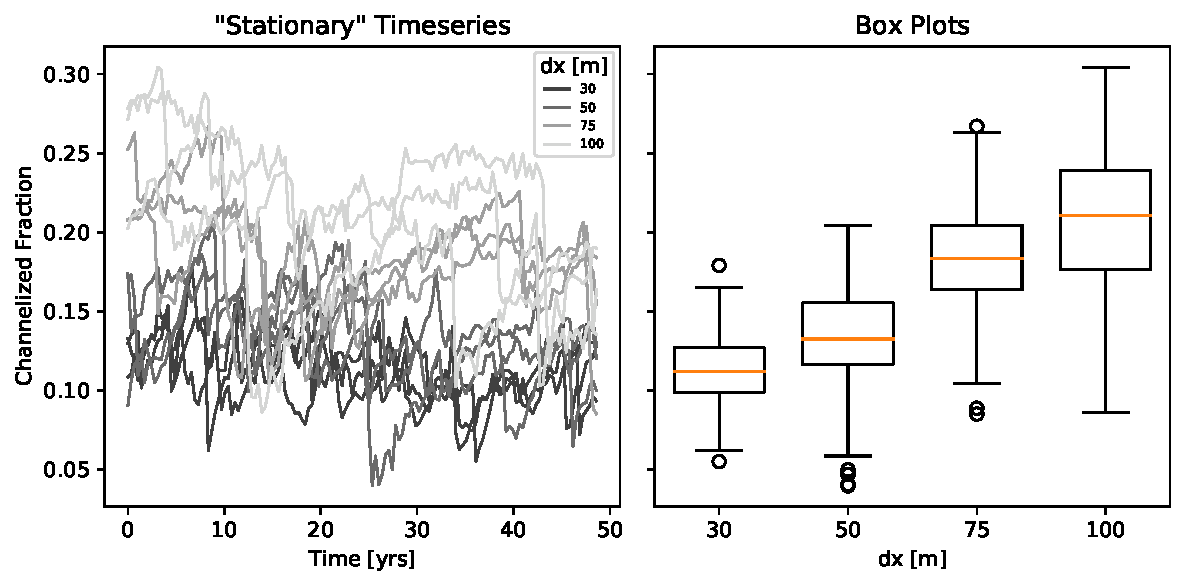
\includegraphics[width=\textwidth]{CellResAnalysis/figs/chanfrac_stationary.pdf}
	}	
	\caption{Channelized fraction values for the final 50 years of each simulation (Left), and box plots of those values for each cell resolution tested (Right).}
	\label{fig:res_chanfrac}
\end{figure}

\begin{figure}[!ht]
	\makebox[\textwidth][c]{
	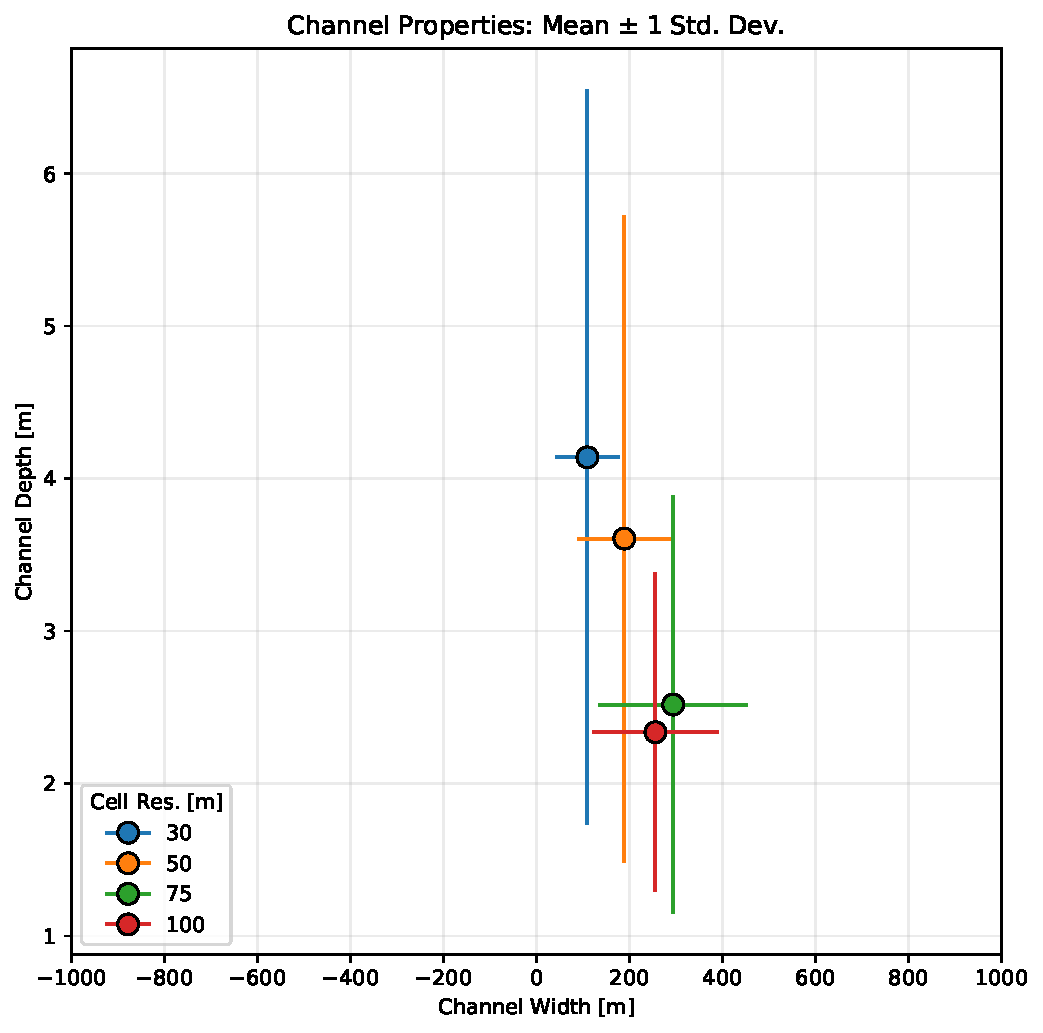
\includegraphics[width=\textwidth]{CellResAnalysis/figs/depth_v_width.pdf}
	}	
	\caption{Plots of average channel depth vs average channel width values as calculated along the azimuthal transects.}
	\label{fig:res_depth_v_width}
\end{figure}

\begin{figure}[!ht]
	\makebox[\textwidth][c]{
	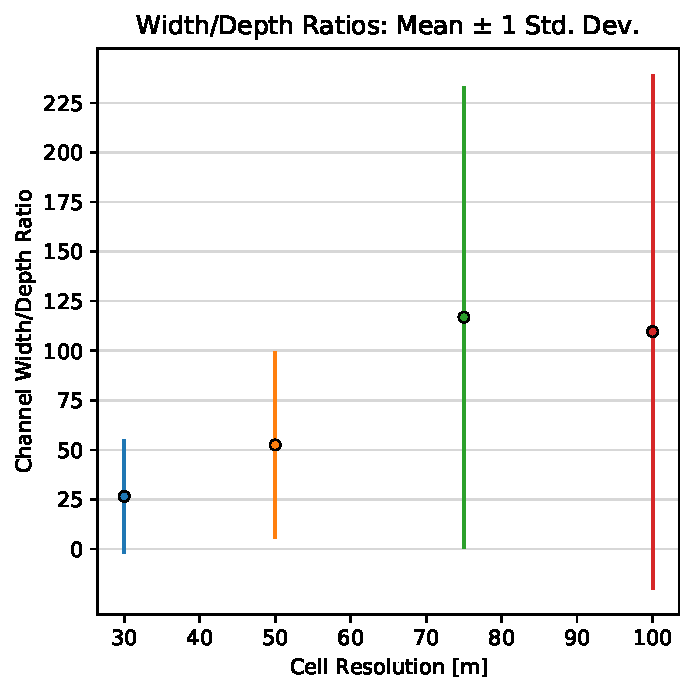
\includegraphics[width=\textwidth]{CellResAnalysis/figs/widthdepth_ratio.pdf}
	}	
	\caption{Width-to-depth ratios of the surface channels as a function of model cell resolution.}
	\label{fig:res_wd}
\end{figure}

\section{Conclusions}
Model cell resolution does not only impact the time it takes to run the model, surface properties are impacted as well.
As the model grid resolution becomes more coarse, channel width-to-depth ratios increase as the channels are forced to widths which are multiples of the grid resolution, although the input conditions are unchanged.
The fraction of the surface that is channelized increases as the model becomes more coarse for a similar reason.
It is therefore important to think about the resolution of the cells when designing a pyDeltaRCM model run; for larger deltas it may be acceptable to move to a coarser cell resolution, but for small ``Wax Lake-like" deltas, it is probably not advisable to move to cells any larger than 50m.

\clearpage
\bibliographystyle{plainnat}
\bibliography{bib/bib}

\chapter{Impact of Number of Parcels on Model Results}
\section{Background}
While we have shown that the number of parcels, in particular the number of sediment parcels, can have a significant impact on model runtimes (Chapter \ref{chap:npruntime}), we do not know how the choice of parcel counts impacts the simulation results.

\section{Model Runs}
A bunch of model runs are conducted (in triplicate) using different numbers of water and sediment parcels ranging from as few as 50 parcels of each to as many as 4,000 (default value is 2,000).
These runs are at ``field-scale" using parameters similar to those from previous studies \cite{Liang2016, Liang2016a}.
The YAML below provides basic information about the parameter set used.\\

\noindent \texttt{YAML} configuration file: \vspace{-6pt}
\begin{boxedverbatim}
Length: 7500
Width: 15000
timesteps: 5000
ensemble: 3
L0_meters: 150.0
N0_meters: 250.0
dx: 50.0
h0: 5.0
\end{boxedverbatim}

\section{Results}
Visualizations of final topographies from the different scenarios is provided (Figure \ref{fig:np_finaltopos}).
Slices of stratigraphy (Figure \ref{fig:np_sections}), land and channel masks (Figure \ref{fig:np_masks}), and timeseries of some surface propertes (Figure \ref{fig:np_surfmetrics}) are provided for subsets of these runs.
The channelized fraction metric is evaluated over the final 25 years for each scenario and aggregated into boxplots to more easily compare the influence of the parcel counts on surface morphology (Figure \ref{fig:np_boxplots}).
Along sections with 2km radii (Figure \ref{fig:np_radial}), width-to-depth ratios of the surface channels are calculated and provided for each individual model run, grouped by the number of parcels (Figure \ref{fig:np_wd_box}).

\begin{sidewaysfigure}[!ht]
	\makebox[\textwidth][c]{
	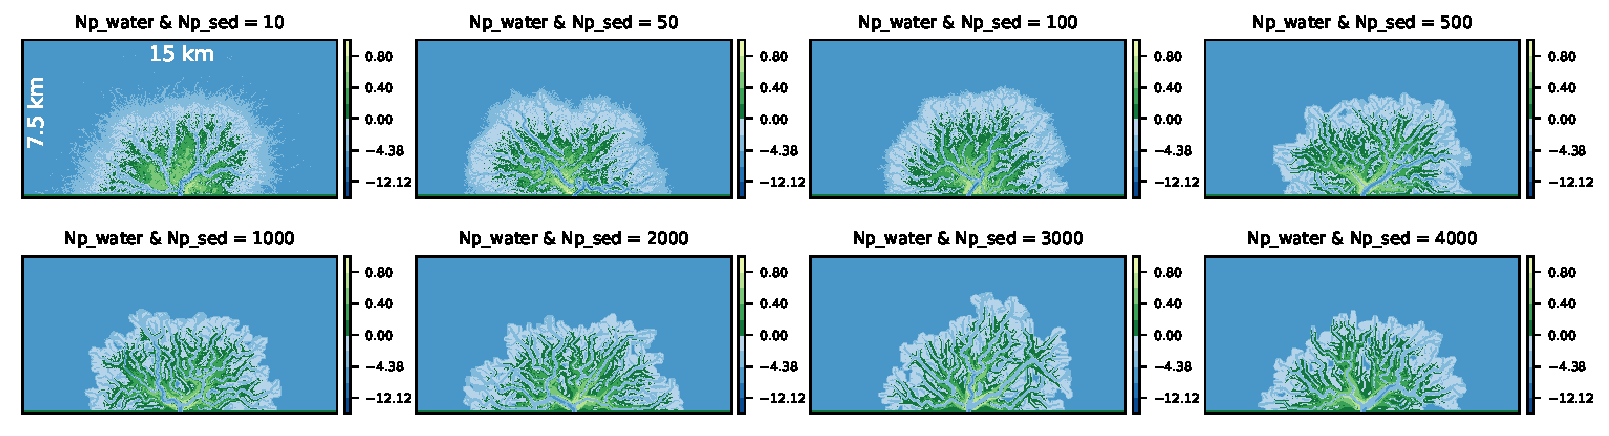
\includegraphics[width=\textwidth]{ParcelNumAnalysis/figs/full_varying_npboth.pdf}
	}	
	\caption{Final topographies when different numbers of parcels are used.}
	\label{fig:np_finaltopos}
\end{sidewaysfigure}

\begin{figure}[!ht]
	\makebox[\textwidth][c]{
	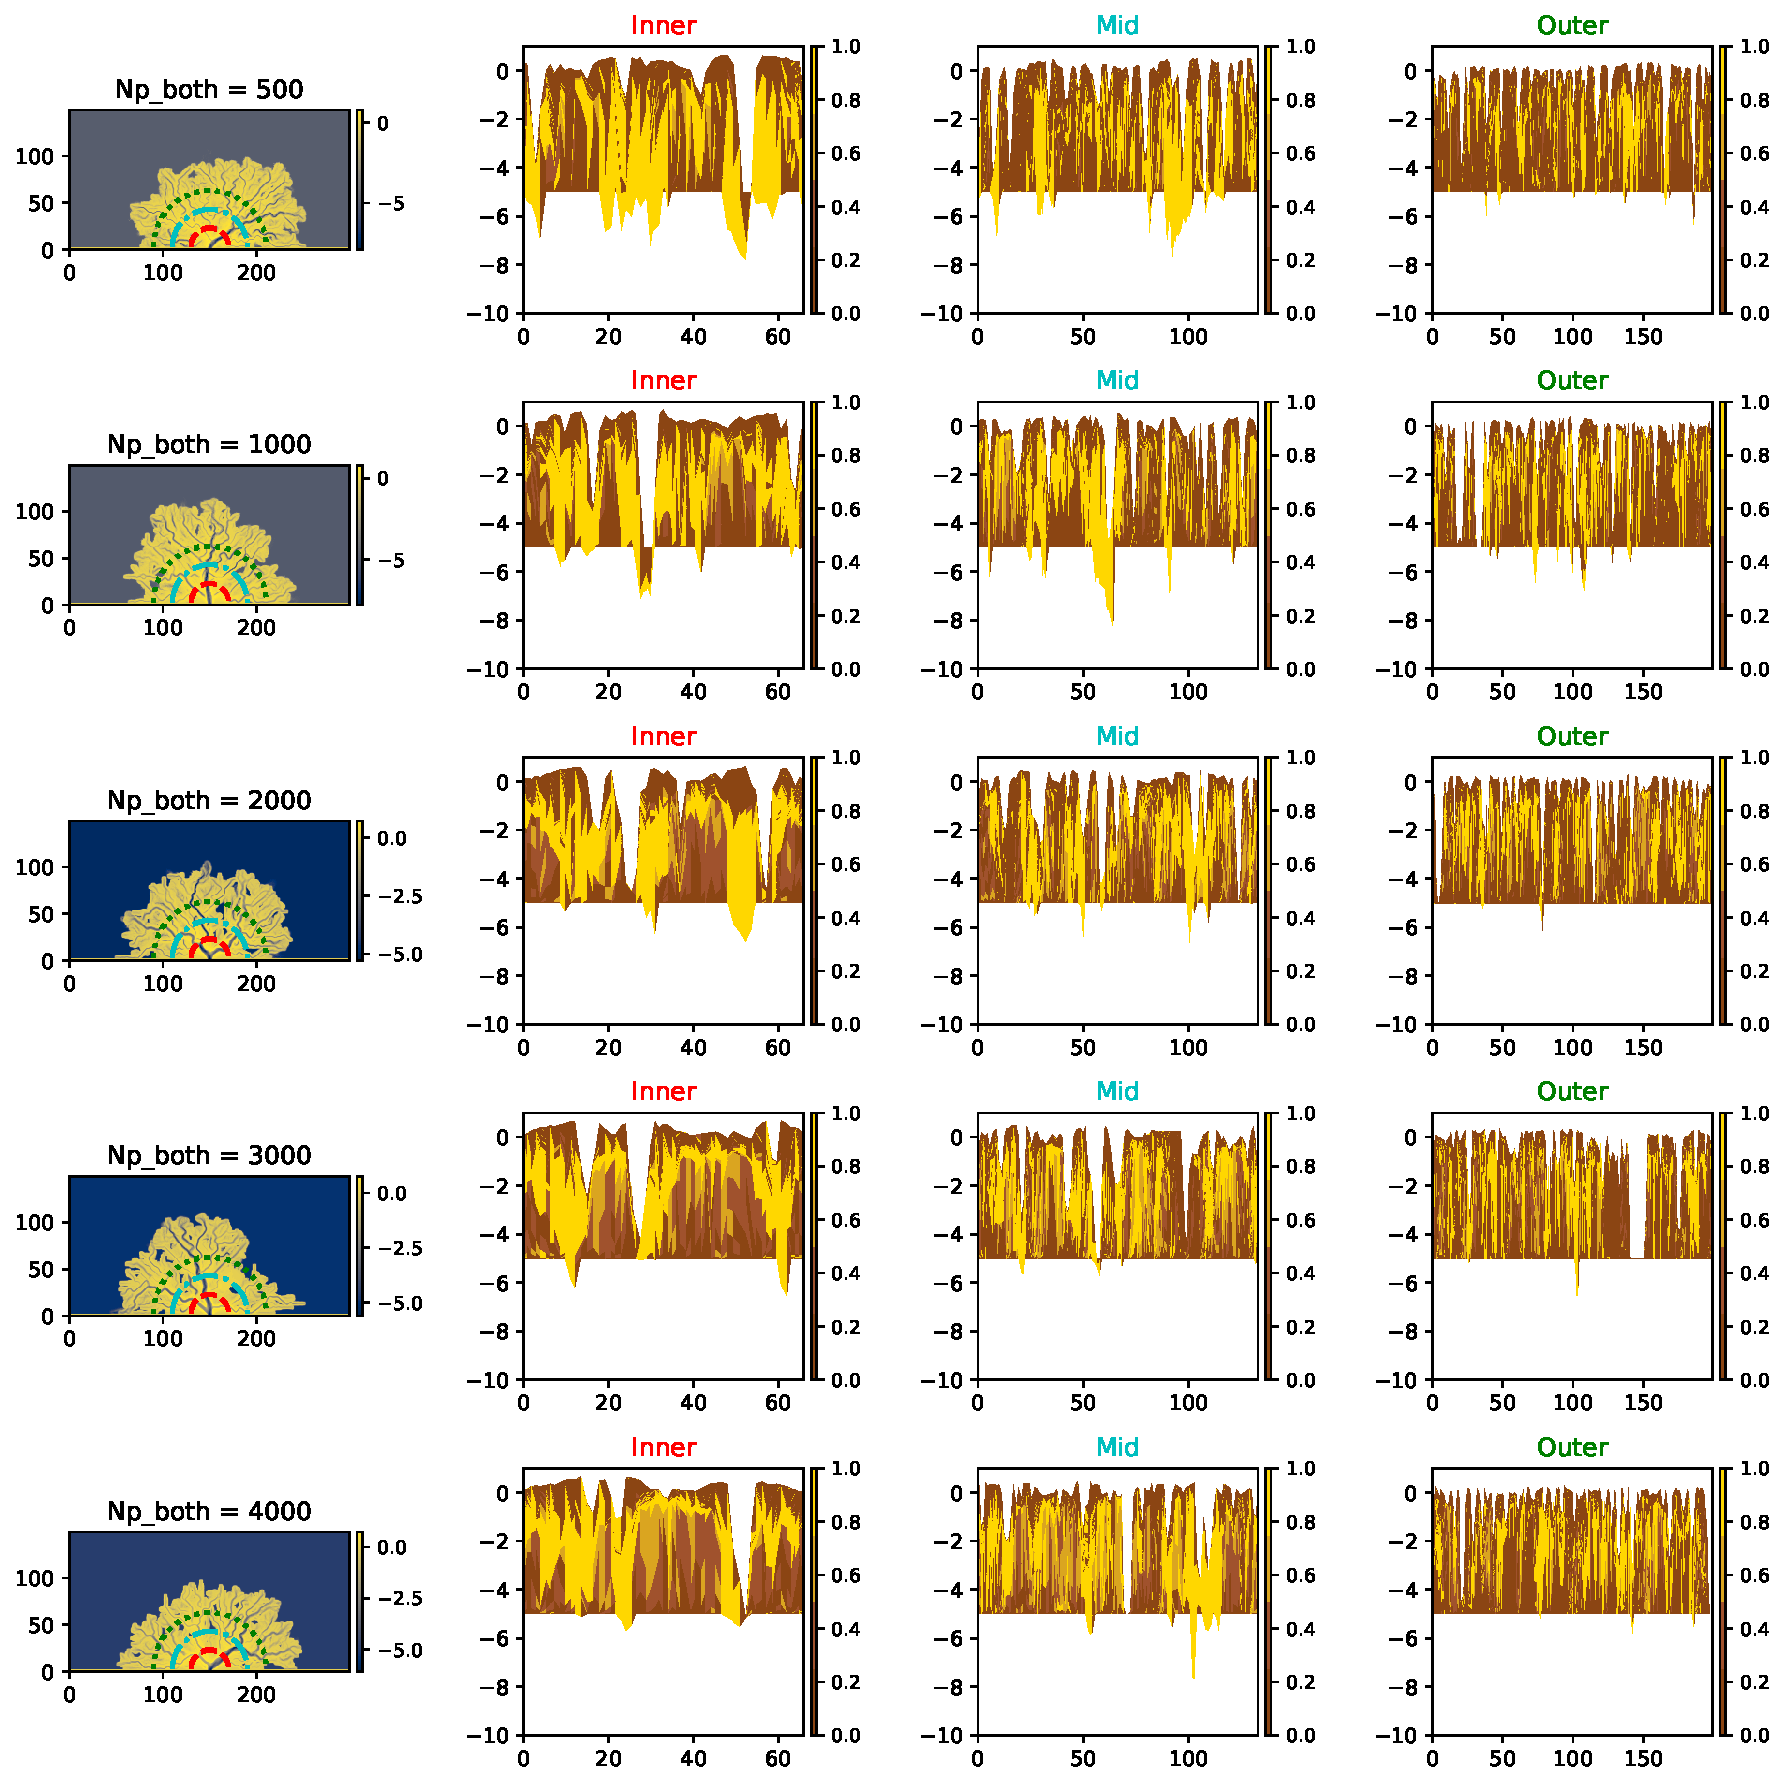
\includegraphics[width=\textwidth]{ParcelNumAnalysis/figs/npboth_sections.pdf}
	}	
	\caption{Sample topographic sections.}
	\label{fig:np_sections}
\end{figure}

\begin{figure}[!ht]
	\makebox[\textwidth][c]{
	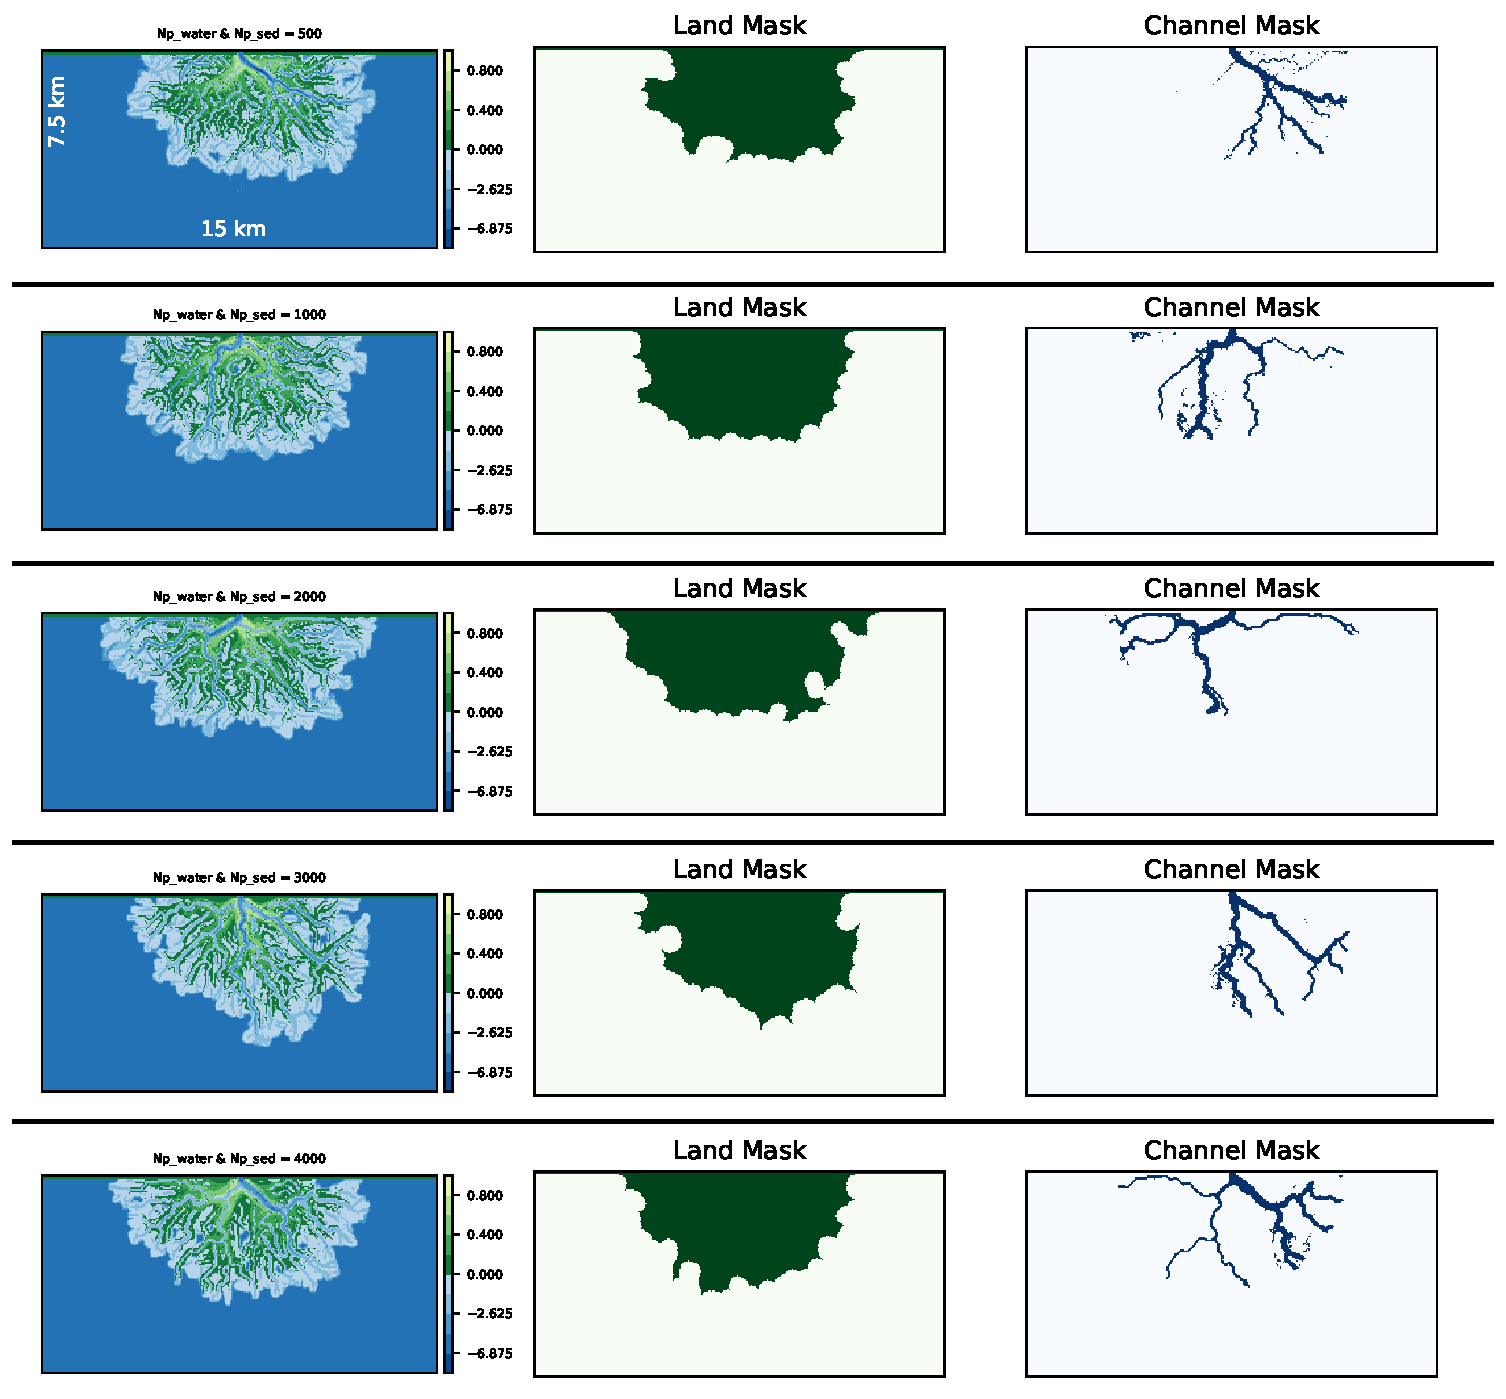
\includegraphics[width=\textwidth]{ParcelNumAnalysis/figs/varying_npboth_viz.pdf}
	}	
	\caption{Visuals of land masks and channel masks with their source topographies.}
	\label{fig:np_masks}
\end{figure}

\begin{sidewaysfigure}[!ht]
	\makebox[\textwidth][c]{
	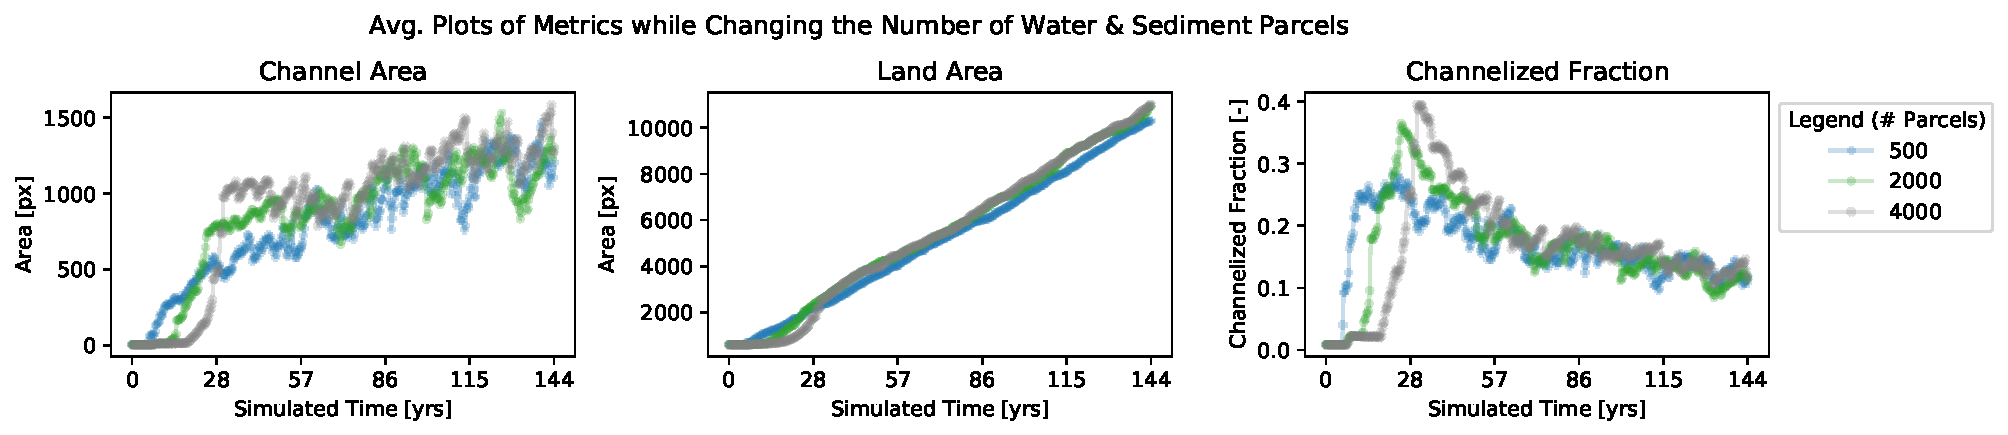
\includegraphics[width=\textwidth]{ParcelNumAnalysis/figs/npboth_avgmetrics_subset.pdf}
	}	
	\caption{Surface metric timeseries for three of the cases.}
	\label{fig:np_surfmetrics}
\end{sidewaysfigure}

\begin{figure}[!ht]
	\makebox[\textwidth][c]{
	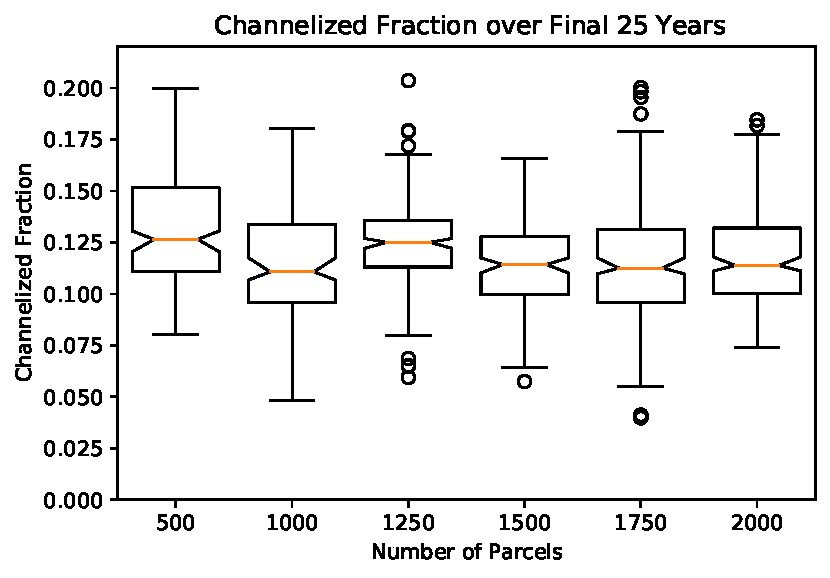
\includegraphics[width=\textwidth]{ParcelNumAnalysis/figs/midnp_cfrac_box.pdf}
	}	
	\caption{Box plots for the final 25 years split by parcel counts.}
	\label{fig:np_boxplots}
\end{figure}

\begin{figure}[!ht]
	\makebox[\textwidth][c]{
	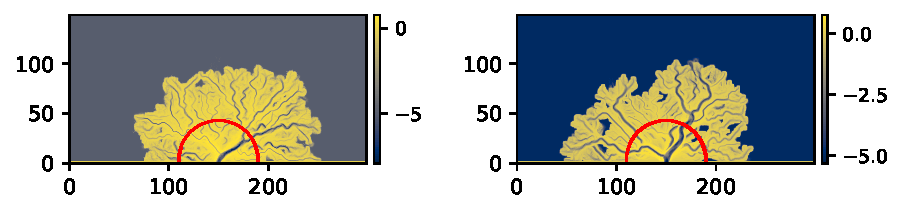
\includegraphics[width=\textwidth]{ParcelNumAnalysis/figs/midnp_sec.pdf}
	}	
	\caption{Visual of 2km azimuthal section locations.}
	\label{fig:np_radial}
\end{figure}

\begin{figure}[!ht]
	\makebox[\textwidth][c]{
	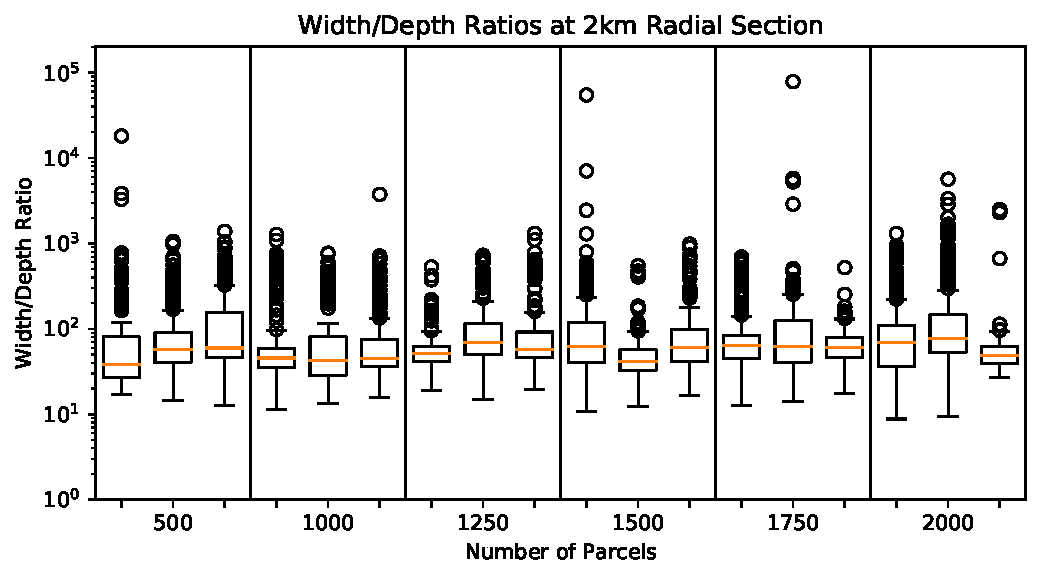
\includegraphics[width=\textwidth]{ParcelNumAnalysis/figs/midnp_widdep_box.pdf}
	}	
	\caption{Box plots of width-to-depth ratios for individual model runs grouped by parcel counts.}
	\label{fig:np_wd_box}
\end{figure}

\section{Conclusions}
Surprisingly, there are few obvious differences due to parcel numbers across the measured metrics.
When parcel numbers get really low (e.g., 50 parcels) it is clear that the model suffers; however once parcel counts get up to 500, especially once they reach 1,000 and greater, the models become very similar to each other.
This implies that we can push the model and get faster results by dropping parcel counts to 1,000 parcels rather than the 2,000 default value with little to no repercussions.

\clearpage
\bibliographystyle{plainnat}
\bibliography{bib/bib}

\chapter{Inlet Discharge and Channel Geometry}
\section{Background}
The relationship between input discharge (both water and sediment) and the resulting channel properties such as the channel width-to-depth ratio is unknown for the DeltaRCM model. 

\section{Model Runs}
A set of 7 model runs, each with a different input discharge are conducted by modifying the depth of the inlet, which alters the discharge fed into the domain without increasing the inlet width.
These runs are at ``field-scale" using parameters similar to those from previous studies \cite{Liang2016, Liang2016a}.
The YAML below provides information about the parameter set used.\\

\noindent \texttt{YAML} configuration file: \vspace{-6pt}
\begin{boxedverbatim}
timesteps: 5000
Length: 10000.0
Width: 22000.0
L0_meters: 150.0  # will be 3 cells (the minimum)
N0_meters: 250.0
hb: 5.0
dx: 100.0
SLR: 36e-10  # small background SLR
Np_water: 2000
Np_sed: 2000
save_dt: 250000

matrix:
  h0:
    - 4.0  # shallower than basin
    - 5.0  # same as basin
    - 6.0
    - 7.0
    - 8.0
    - 9.0
    - 10.0  # double basin
\end{boxedverbatim}

\section{Results}

\begin{figure}[!ht]
	\makebox[\textwidth][c]{
	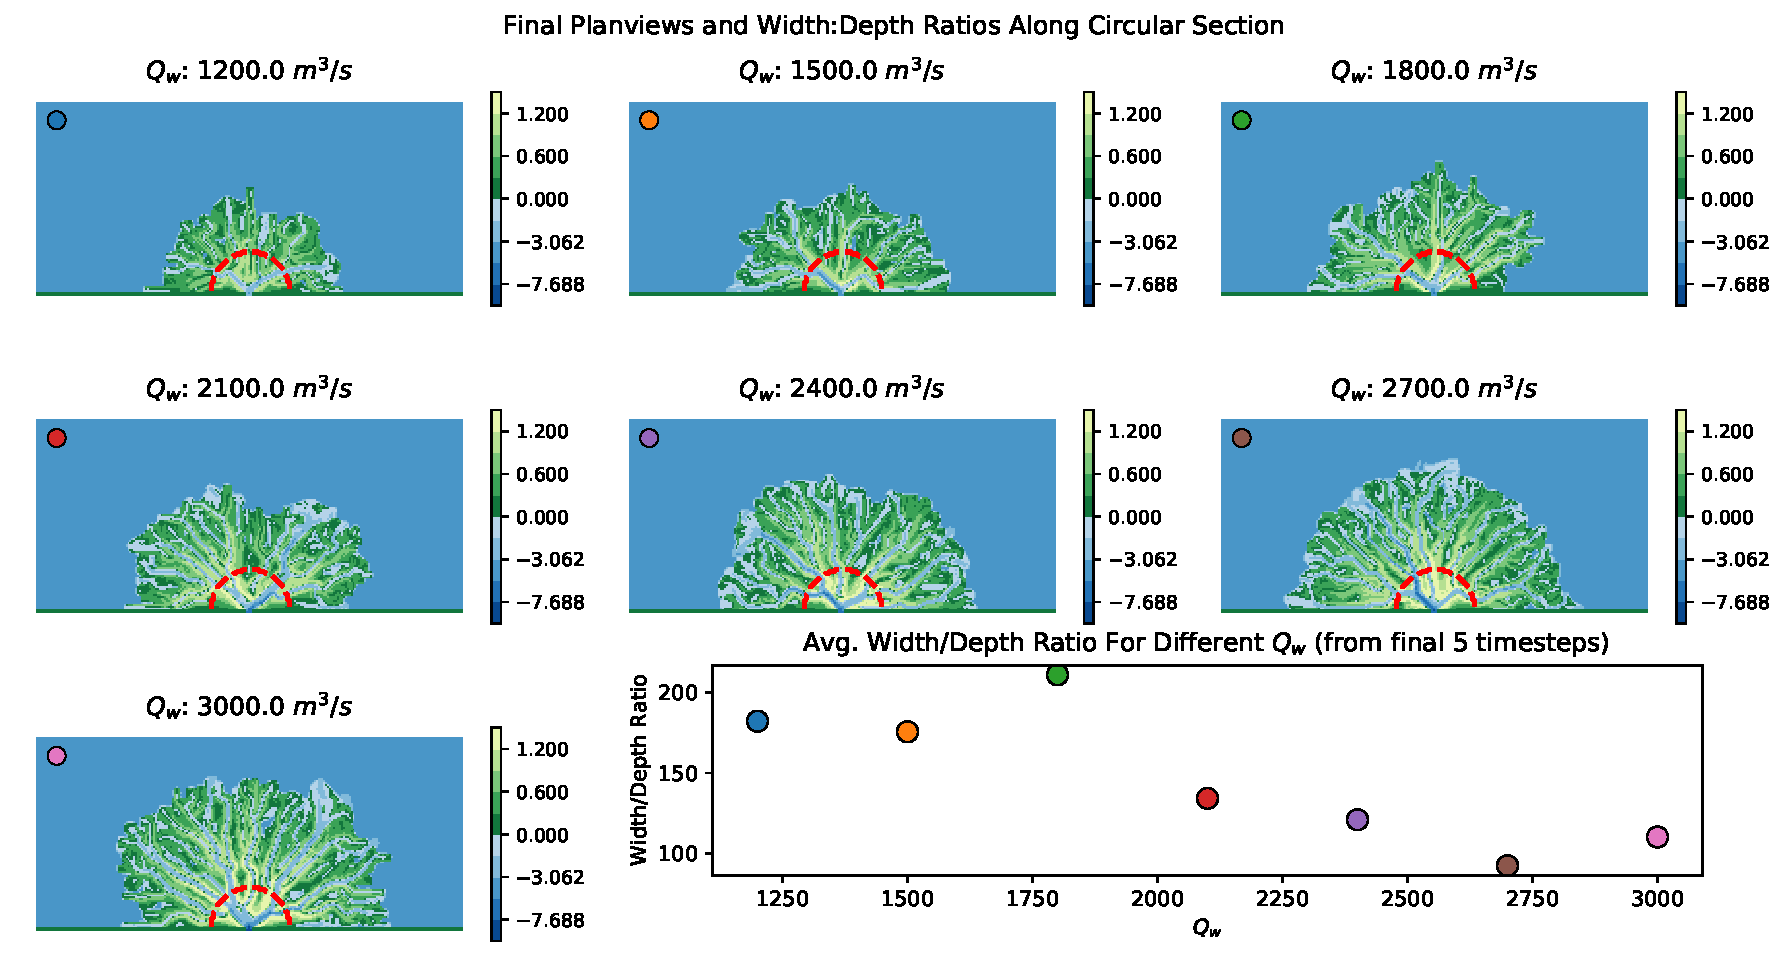
\includegraphics[width=\textwidth]{QandWidthDepth/figs/FinalPlans_WidthDepth.pdf}
	}	
	\caption{Final model topographies from the 7 runs generated by the YAML configuration file. Bottom right plot shows the average width-to-depth ratios of the channels along the circular sections shown in red, using data from the last 5 timesteps of each run.}
	\label{fig:QWD_plot}
\end{figure}

\section{Conclusions}
Unsurprisingly as the input discharge value is increased the size of the resulting delta increases. There is also an observed decrease in the width-to-depth ratios of the channels as the inlet discharge increases. 

\bibliographystyle{plainnat}
\bibliography{bib/bib}

% include appendices
\appendix

\chapter{Model Comparison - Final Topographies}

\begin{figure}[!ht]
	\makebox[\textwidth][c]{
	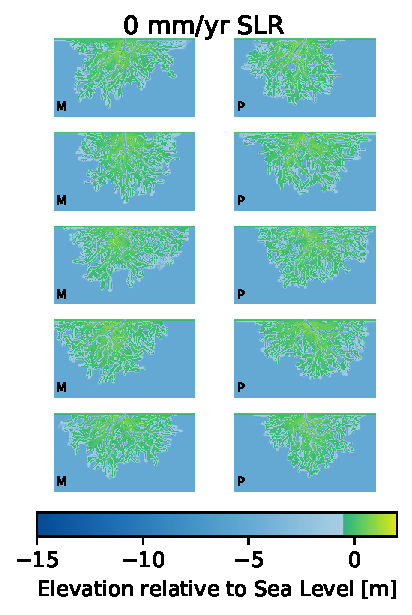
\includegraphics[height=0.95\textheight]{DeltaRCM_ModelComparison/figs/000Topo.pdf}
	}
	\caption{Final topographies for 0 mm/yr replicates. Domain has been clipped.}
	\label{fig:000topo}
\end{figure}

\begin{figure}[!ht]
	\makebox[\textwidth][c]{
	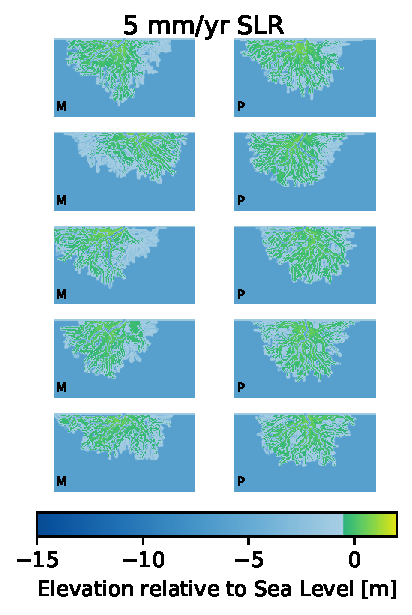
\includegraphics[height=0.95\textheight]{DeltaRCM_ModelComparison/figs/005Topo.pdf}
	}
	\caption{Final topographies for 5 mm/yr replicates. Domain has been clipped.}
	\label{fig:005topo}
\end{figure}

\begin{figure}[!ht]
	\makebox[\textwidth][c]{
	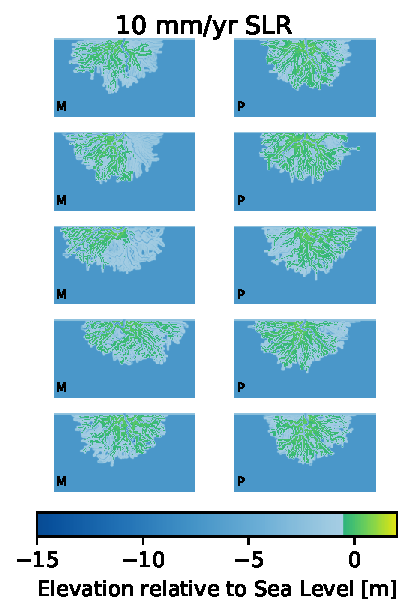
\includegraphics[height=0.95\textheight]{DeltaRCM_ModelComparison/figs/010Topo.pdf}
	}
	\caption{Final topographies for 10 mm/yr replicates. Domain has been clipped.}
	\label{fig:010topo}
\end{figure}

\begin{figure}[!ht]
	\makebox[\textwidth][c]{
	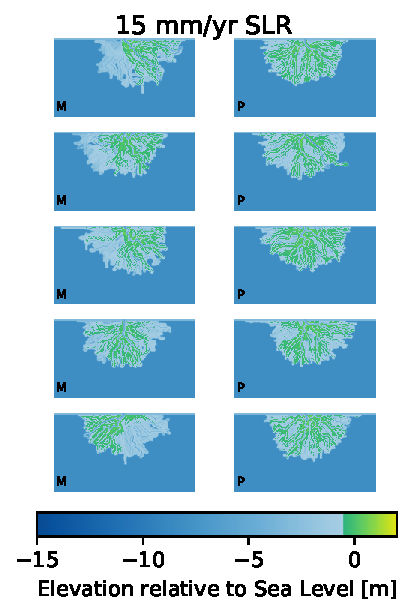
\includegraphics[height=0.95\textheight]{DeltaRCM_ModelComparison/figs/015Topo.pdf}
	}
	\caption{Final topographies for 15 mm/yr replicates. Domain has been clipped.}
	\label{fig:015topo}
\end{figure}

\begin{figure}[!ht]
	\makebox[\textwidth][c]{
	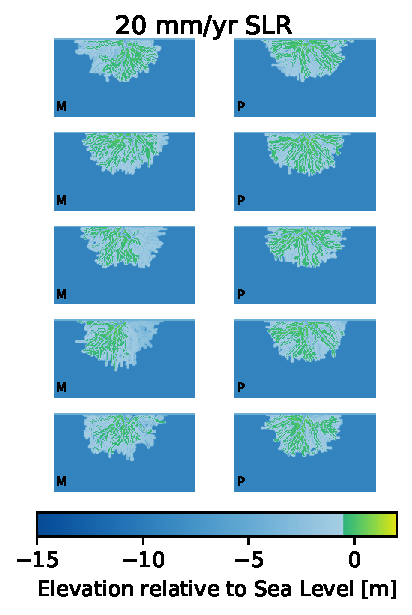
\includegraphics[height=0.95\textheight]{DeltaRCM_ModelComparison/figs/020Topo.pdf}
	}
	\caption{Final topographies for 20 mm/yr replicates. Domain has been clipped.}
	\label{fig:020topo}
\end{figure}

\begin{figure}[!ht]
	\makebox[\textwidth][c]{
	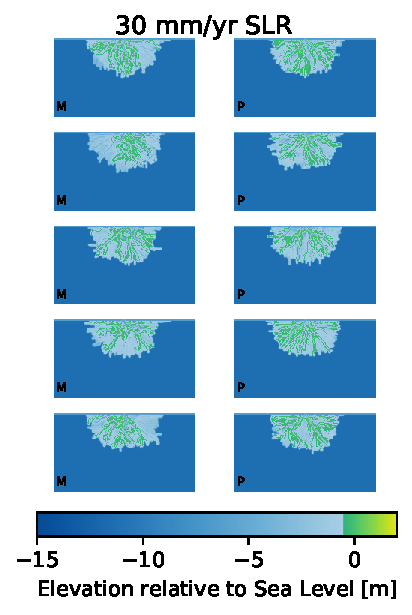
\includegraphics[height=0.95\textheight]{DeltaRCM_ModelComparison/figs/030Topo.pdf}
	}
	\caption{Final topographies for 30 mm/yr replicates. Domain has been clipped.}
	\label{fig:030topo}
\end{figure}

\begin{figure}[!ht]
	\makebox[\textwidth][c]{
	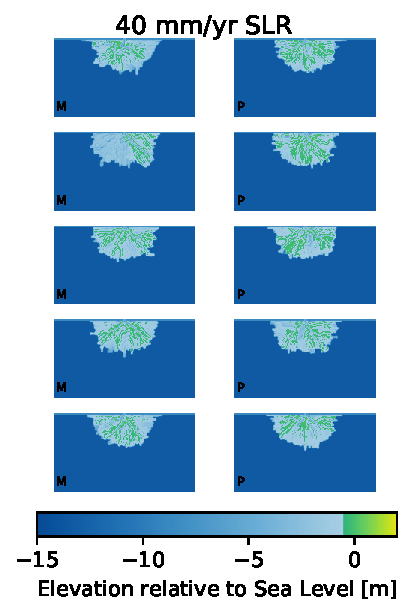
\includegraphics[height=0.95\textheight]{DeltaRCM_ModelComparison/figs/040Topo.pdf}
	}
	\caption{Final topographies for 40 mm/yr replicates. Domain has been clipped.}
	\label{fig:040topo}
\end{figure}

\end{document}